% Options for packages loaded elsewhere
% Options for packages loaded elsewhere
\PassOptionsToPackage{unicode}{hyperref}
\PassOptionsToPackage{hyphens}{url}
\PassOptionsToPackage{dvipsnames,svgnames,x11names}{xcolor}
%
\documentclass[
  10pt]{article}
\usepackage{xcolor}
\usepackage{amsmath,amssymb}
\setcounter{secnumdepth}{5}
\usepackage{iftex}
\ifPDFTeX
  \usepackage[T1]{fontenc}
  \usepackage[utf8]{inputenc}
  \usepackage{textcomp} % provide euro and other symbols
\else % if luatex or xetex
  \usepackage{unicode-math} % this also loads fontspec
  \defaultfontfeatures{Scale=MatchLowercase}
  \defaultfontfeatures[\rmfamily]{Ligatures=TeX,Scale=1}
\fi
\usepackage{lmodern}
\ifPDFTeX\else
  % xetex/luatex font selection
\fi
% Use upquote if available, for straight quotes in verbatim environments
\IfFileExists{upquote.sty}{\usepackage{upquote}}{}
\IfFileExists{microtype.sty}{% use microtype if available
  \usepackage[]{microtype}
  \UseMicrotypeSet[protrusion]{basicmath} % disable protrusion for tt fonts
}{}
\makeatletter
\@ifundefined{KOMAClassName}{% if non-KOMA class
  \IfFileExists{parskip.sty}{%
    \usepackage{parskip}
  }{% else
    \setlength{\parindent}{0pt}
    \setlength{\parskip}{6pt plus 2pt minus 1pt}}
}{% if KOMA class
  \KOMAoptions{parskip=half}}
\makeatother
% Make \paragraph and \subparagraph free-standing
\makeatletter
\ifx\paragraph\undefined\else
  \let\oldparagraph\paragraph
  \renewcommand{\paragraph}{
    \@ifstar
      \xxxParagraphStar
      \xxxParagraphNoStar
  }
  \newcommand{\xxxParagraphStar}[1]{\oldparagraph*{#1}\mbox{}}
  \newcommand{\xxxParagraphNoStar}[1]{\oldparagraph{#1}\mbox{}}
\fi
\ifx\subparagraph\undefined\else
  \let\oldsubparagraph\subparagraph
  \renewcommand{\subparagraph}{
    \@ifstar
      \xxxSubParagraphStar
      \xxxSubParagraphNoStar
  }
  \newcommand{\xxxSubParagraphStar}[1]{\oldsubparagraph*{#1}\mbox{}}
  \newcommand{\xxxSubParagraphNoStar}[1]{\oldsubparagraph{#1}\mbox{}}
\fi
\makeatother

\usepackage{color}
\usepackage{fancyvrb}
\newcommand{\VerbBar}{|}
\newcommand{\VERB}{\Verb[commandchars=\\\{\}]}
\DefineVerbatimEnvironment{Highlighting}{Verbatim}{commandchars=\\\{\}}
% Add ',fontsize=\small' for more characters per line
\usepackage{framed}
\definecolor{shadecolor}{RGB}{241,243,245}
\newenvironment{Shaded}{\begin{snugshade}}{\end{snugshade}}
\newcommand{\AlertTok}[1]{\textcolor[rgb]{0.68,0.00,0.00}{#1}}
\newcommand{\AnnotationTok}[1]{\textcolor[rgb]{0.37,0.37,0.37}{#1}}
\newcommand{\AttributeTok}[1]{\textcolor[rgb]{0.40,0.45,0.13}{#1}}
\newcommand{\BaseNTok}[1]{\textcolor[rgb]{0.68,0.00,0.00}{#1}}
\newcommand{\BuiltInTok}[1]{\textcolor[rgb]{0.00,0.23,0.31}{#1}}
\newcommand{\CharTok}[1]{\textcolor[rgb]{0.13,0.47,0.30}{#1}}
\newcommand{\CommentTok}[1]{\textcolor[rgb]{0.37,0.37,0.37}{#1}}
\newcommand{\CommentVarTok}[1]{\textcolor[rgb]{0.37,0.37,0.37}{\textit{#1}}}
\newcommand{\ConstantTok}[1]{\textcolor[rgb]{0.56,0.35,0.01}{#1}}
\newcommand{\ControlFlowTok}[1]{\textcolor[rgb]{0.00,0.23,0.31}{\textbf{#1}}}
\newcommand{\DataTypeTok}[1]{\textcolor[rgb]{0.68,0.00,0.00}{#1}}
\newcommand{\DecValTok}[1]{\textcolor[rgb]{0.68,0.00,0.00}{#1}}
\newcommand{\DocumentationTok}[1]{\textcolor[rgb]{0.37,0.37,0.37}{\textit{#1}}}
\newcommand{\ErrorTok}[1]{\textcolor[rgb]{0.68,0.00,0.00}{#1}}
\newcommand{\ExtensionTok}[1]{\textcolor[rgb]{0.00,0.23,0.31}{#1}}
\newcommand{\FloatTok}[1]{\textcolor[rgb]{0.68,0.00,0.00}{#1}}
\newcommand{\FunctionTok}[1]{\textcolor[rgb]{0.28,0.35,0.67}{#1}}
\newcommand{\ImportTok}[1]{\textcolor[rgb]{0.00,0.46,0.62}{#1}}
\newcommand{\InformationTok}[1]{\textcolor[rgb]{0.37,0.37,0.37}{#1}}
\newcommand{\KeywordTok}[1]{\textcolor[rgb]{0.00,0.23,0.31}{\textbf{#1}}}
\newcommand{\NormalTok}[1]{\textcolor[rgb]{0.00,0.23,0.31}{#1}}
\newcommand{\OperatorTok}[1]{\textcolor[rgb]{0.37,0.37,0.37}{#1}}
\newcommand{\OtherTok}[1]{\textcolor[rgb]{0.00,0.23,0.31}{#1}}
\newcommand{\PreprocessorTok}[1]{\textcolor[rgb]{0.68,0.00,0.00}{#1}}
\newcommand{\RegionMarkerTok}[1]{\textcolor[rgb]{0.00,0.23,0.31}{#1}}
\newcommand{\SpecialCharTok}[1]{\textcolor[rgb]{0.37,0.37,0.37}{#1}}
\newcommand{\SpecialStringTok}[1]{\textcolor[rgb]{0.13,0.47,0.30}{#1}}
\newcommand{\StringTok}[1]{\textcolor[rgb]{0.13,0.47,0.30}{#1}}
\newcommand{\VariableTok}[1]{\textcolor[rgb]{0.07,0.07,0.07}{#1}}
\newcommand{\VerbatimStringTok}[1]{\textcolor[rgb]{0.13,0.47,0.30}{#1}}
\newcommand{\WarningTok}[1]{\textcolor[rgb]{0.37,0.37,0.37}{\textit{#1}}}

\usepackage{longtable,booktabs,array}
\newcounter{none} % for unnumbered tables
\usepackage{calc} % for calculating minipage widths
% Correct order of tables after \paragraph or \subparagraph
\usepackage{etoolbox}
\makeatletter
\patchcmd\longtable{\par}{\if@noskipsec\mbox{}\fi\par}{}{}
\makeatother
% Allow footnotes in longtable head/foot
\IfFileExists{footnotehyper.sty}{\usepackage{footnotehyper}}{\usepackage{footnote}}
\makesavenoteenv{longtable}
\usepackage{graphicx}
\makeatletter
\newsavebox\pandoc@box
\newcommand*\pandocbounded[1]{% scales image to fit in text height/width
  \sbox\pandoc@box{#1}%
  \Gscale@div\@tempa{\textheight}{\dimexpr\ht\pandoc@box+\dp\pandoc@box\relax}%
  \Gscale@div\@tempb{\linewidth}{\wd\pandoc@box}%
  \ifdim\@tempb\p@<\@tempa\p@\let\@tempa\@tempb\fi% select the smaller of both
  \ifdim\@tempa\p@<\p@\scalebox{\@tempa}{\usebox\pandoc@box}%
  \else\usebox{\pandoc@box}%
  \fi%
}
% Set default figure placement to htbp
\def\fps@figure{htbp}
\makeatother





\setlength{\emergencystretch}{3em} % prevent overfull lines

\providecommand{\tightlist}{%
  \setlength{\itemsep}{0pt}\setlength{\parskip}{0pt}}



 
\usepackage[]{natbib}
\bibliographystyle{agsm}


\usepackage{geometry}
\geometry{margin=0.85in}
\makeatletter
\@ifpackageloaded{caption}{}{\usepackage{caption}}
\AtBeginDocument{%
\ifdefined\contentsname
  \renewcommand*\contentsname{Table of contents}
\else
  \newcommand\contentsname{Table of contents}
\fi
\ifdefined\listfigurename
  \renewcommand*\listfigurename{List of Figures}
\else
  \newcommand\listfigurename{List of Figures}
\fi
\ifdefined\listtablename
  \renewcommand*\listtablename{List of Tables}
\else
  \newcommand\listtablename{List of Tables}
\fi
\ifdefined\figurename
  \renewcommand*\figurename{Figure}
\else
  \newcommand\figurename{Figure}
\fi
\ifdefined\tablename
  \renewcommand*\tablename{Table}
\else
  \newcommand\tablename{Table}
\fi
}
\@ifpackageloaded{float}{}{\usepackage{float}}
\floatstyle{ruled}
\@ifundefined{c@chapter}{\newfloat{codelisting}{h}{lop}}{\newfloat{codelisting}{h}{lop}[chapter]}
\floatname{codelisting}{Listing}
\newcommand*\listoflistings{\listof{codelisting}{List of Listings}}
\makeatother
\makeatletter
\makeatother
\makeatletter
\@ifpackageloaded{caption}{}{\usepackage{caption}}
\@ifpackageloaded{subcaption}{}{\usepackage{subcaption}}
\makeatother
\usepackage{bookmark}
\IfFileExists{xurl.sty}{\usepackage{xurl}}{} % add URL line breaks if available
\urlstyle{same}
% fallback for those not using the hyperref driver hyperxmp:
\makeatletter
\@ifundefined{xmpquote}{\newcommand{\xmpquote}[1]{#1}}{}
\makeatother
\hypersetup{
  pdftitle={Start Strong: An Analysis of Motorsport Qualifying with a Novel Python Package},
  pdfauthor={Anonymous},
  pdfkeywords={\xmpquote{Motorsports}, \xmpquote{IndyCar}, \xmpquote{Formula
1}, \xmpquote{NASCAR}, \xmpquote{Qualifying}, \xmpquote{Sports
Analytics}},
  colorlinks=true,
  linkcolor={blue},
  filecolor={Maroon},
  citecolor={Blue},
  urlcolor={Blue},
  pdfcreator={LaTeX via pandoc}}



\begin{document}


\def\spacingset#1{\renewcommand{\baselinestretch}%
{#1}\small\normalsize} \spacingset{1}


%%%%%%%%%%%%%%%%%%%%%%%%%%%%%%%%%%%%%%%%%%%%%%%%%%%%%%%%%%%%%%%%%%%%%%%%%%%%%%

\date{September 4, 2026}
\title{\bf Start Strong: An Analysis of Motorsport Qualifying with a
Novel Python Package}
\author{
Anonymous\\
{[}Institution Name{]}\\
}
\maketitle

\bigskip
\bigskip
\begin{abstract}
Competitive motorsports are unique compared to other sports because,
through qualifying, an advantage can be gained before the day of the
event. However, the extent of qualifying's advantage can differ heavily
across race series. To quantify these differences, lap-by-lap data were
obtained using the Python libraries FastF1 and PyNascar. A new
pip-installable package called RaceIndyCar was created in order to
provide accessible access to IndyCar. The official IndyCar.com website
was scraped for start position, finish position, average speed, and more
for the package. Individual track section speeds and times are also
included for every lap of every race since 2013. Then, for an analysis
of all three series, two regression models were deployed. One uses
driver quality and race-specific fixed effects, and the other adds the
qualifying position to the same model. Expressed as partial R²,
qualifying explains approximately 17\% of the variation that driver
quality does not already explain in F1, compared with 7\% in IndyCar and
4\% in NASCAR. This research shows that F1 teams should focus more on
the strategy for qualifying as opposed to IndyCar and NASCAR teams, who
should focus more on improving their car for race day, even if it means
performing worse in qualifying.
\end{abstract}

\noindent%
{\it Keywords:} Motorsports, IndyCar, Formula
1, NASCAR, Qualifying, Sports Analytics
\vfill

\spacingset{1} % DON'T change the spacing!


\section{Introduction}\label{introduction}

Competitive motorsports are unique compared to other sports because,
through qualifying, an advantage can be gained before the day of the
event. Formula 1 (F1), NASCAR, and IndyCar all hold qualifying sessions
that, on the surface, appear to have varying effects on the results of
the race. For example, take two seven-time champions of their respective
series: Lewis Hamilton (F1) and Jimmie Johnson (NASCAR). 61 of Lewis
Hamilton's 106 race wins \citep{statsf1_hamilton} came from pole
position, compared to a mere 15 of Jimmie Johnson's 83 wins
\citep{motorsportstats_johnson}, pointing to potentially drastic
differences in the relative importance of qualifying across race series.

So, we aim to quantify the relative importance of qualifying between
these three major race series. In doing so, we create a new
pip-installable Python package for obtaining lap-by-lap IndyCar data,
which was previously unobtainable. Using lap-level information for each
series, we adjust for driver performance to isolate the effects and try
to gain actionable insight into the differences in race weekend
operations across series.

\subsection{Data Collection}\label{data-collection}

Data was obtained using the FastF1 and PyNascar Python libraries. The
custom package described below, RaceIndyCar, was created to obtain
lap-by-lap data for IndyCar. For each race, general statistics such as
start position, finish position, average speed, and more are kept.
Additionally, we obtain data for each lap of every race, including each
driver's position, lap speed, and lap time.

\section{RaceIndyCar Package}\label{raceindycar-package}

\subsection{Introduction}\label{introduction-1}

RaceIndyCar is pip installable, or available on
\href{https://pypi.org/project/raceindycar}{PyPI}.

\begin{Shaded}
\begin{Highlighting}[]
\NormalTok{pip install raceindycar}
\end{Highlighting}
\end{Shaded}

Requires Python 3.10+. Dependencies (\texttt{pandas}, \texttt{requests},
\texttt{requests-cache}, \texttt{pdfplumber}, \texttt{matplotlib}) are
installed automatically.

In an IndyCar season, there are around 17 race events that occur. Each
race event typically spans a weekend, where within that event there are
individual sessions (such as practices, qualifying, and the race
itself). We scrape information from the official
\href{https://www.indycar.com/}{IndyCar} website and use this idea of
events and sessions in our implementation:

\textsubscript{Source:
\href{https://ArchithSharma.github.io/raceindycar_manuscript/index.qmd.html}{Article
Notebook}}

\begin{Shaded}
\begin{Highlighting}[]
\ImportTok{import}\NormalTok{ raceindycar}

\CommentTok{\# Enable caching so downloaded and parsed data can be reused.}
\NormalTok{raceindycar.enable\_cache(cache\_dir}\OperatorTok{=}\StringTok{".cache/raceindycar"}\NormalTok{, cache\_format}\OperatorTok{=}\StringTok{"pickle"}\NormalTok{)}

\CommentTok{\# Get all events for a given year}
\NormalTok{races }\OperatorTok{=}\NormalTok{ raceindycar.get\_season\_events(}\DecValTok{2025}\NormalTok{)}

\CommentTok{\# Returns an Event with attributes for each schedule column.}
\CommentTok{\# The second argument does a fuzzy name match to find an event,}
\CommentTok{\# or use a round number/integer event id found in the schedule.}
\NormalTok{indy25 }\OperatorTok{=}\NormalTok{ raceindycar.get\_event(}\DecValTok{2025}\NormalTok{, }\StringTok{"Indianapolis 500"}\NormalTok{)}

\CommentTok{\# Identify all sessions (such as practices and qualifying) for the event.}
\NormalTok{session\_info }\OperatorTok{=}\NormalTok{ indy25.sessions}

\CommentTok{\# Get a specific session from an event, with the default as the race session.}
\CommentTok{\# The session argument can either be an EventsSessionID or a SessionName string.}
\NormalTok{race\_session }\OperatorTok{=}\NormalTok{ indy25.get\_session(session}\OperatorTok{=}\StringTok{"R"}\NormalTok{)}

\CommentTok{\# Load data for that session.}
\NormalTok{race\_session.load()}

\CommentTok{\# A Pandas DataFrame of race data, including start position,}
\CommentTok{\# finish position, average speed, etc.}
\NormalTok{race\_session.results.sample(n}\OperatorTok{=}\DecValTok{3}\NormalTok{, random\_state}\OperatorTok{=}\DecValTok{314}\NormalTok{).iloc[:, :}\DecValTok{6}\NormalTok{]}
\end{Highlighting}
\end{Shaded}

{\def\LTcaptype{none} % do not increment counter
\begin{longtable}[]{@{}lllllll@{}}
\toprule\noalign{}
& DriverUrl & DriversID & FirstName & LastName & CarNumber &
EventsSessionsDetailsID \\
\midrule\noalign{}
\endhead
\bottomrule\noalign{}
\endlastfoot
1 & /Drivers/David-Malukas & 4636 & David & Malukas & 4 & 118154 \\
26 & /Drivers/Rinus-VeeKay & 4614 & Rinus & VeeKay & 18 & 118179 \\
31 & /Drivers/Kyle-Kirkwood & 4623 & Kyle & Kirkwood & 27 & 118184 \\
\end{longtable}
}

\textsubscript{Source:
\href{https://ArchithSharma.github.io/raceindycar_manuscript/index.qmd.html}{Article
Notebook}}

It is not required to get an event and then get a session from that
event as shown above. We can go straight to a session for a weekend:

\textsubscript{Source:
\href{https://ArchithSharma.github.io/raceindycar_manuscript/index.qmd.html}{Article
Notebook}}

\begin{Shaded}
\begin{Highlighting}[]
\NormalTok{det25\_race }\OperatorTok{=}\NormalTok{ raceindycar.get\_session(}\DecValTok{2025}\NormalTok{, }\StringTok{"Detroit Grand Prix"}\NormalTok{, session}\OperatorTok{=}\StringTok{"R"}\NormalTok{)}
\end{Highlighting}
\end{Shaded}

\textsubscript{Source:
\href{https://ArchithSharma.github.io/raceindycar_manuscript/index.qmd.html}{Article
Notebook}}

From a session, we can obtain the lap-by-lap data, with information on
every section of an IndyCar track. Lap results are scraped from PDFs
that are up to 500 pages long, so loading laps can take anywhere from
30--100 seconds.

\textsubscript{Source:
\href{https://ArchithSharma.github.io/raceindycar_manuscript/index.qmd.html}{Article
Notebook}}

\begin{Shaded}
\begin{Highlighting}[]
\NormalTok{race\_session.load(laps}\OperatorTok{=}\VariableTok{True}\NormalTok{)}

\CommentTok{\# A Pandas DataFrame of each lap, including sectional and position data}
\NormalTok{laps }\OperatorTok{=}\NormalTok{ race\_session.laps}
\NormalTok{laps.sample(n}\OperatorTok{=}\DecValTok{3}\NormalTok{, random\_state}\OperatorTok{=}\DecValTok{314}\NormalTok{).iloc[:, :}\DecValTok{6}\NormalTok{]}
\end{Highlighting}
\end{Shaded}

{\def\LTcaptype{none} % do not increment counter
\begin{longtable}[]{@{}lllllll@{}}
\toprule\noalign{}
& Driver & DriverNumber & LapNumber & Position & LapSpeed & LapTime \\
\midrule\noalign{}
\endhead
\bottomrule\noalign{}
\endlastfoot
3438 & Nolan Siegel & 6 & 169 & 14.0 & 221.034 & 40.7177 \\
2035 & Kyle Kirkwood & 27 & 171 & 12.0 & 223.298 & 40.3049 \\
4519 & Conor Daly & 76 & 58 & 2.0 & 217.388 & 41.4007 \\
\end{longtable}
}

\textsubscript{Source:
\href{https://ArchithSharma.github.io/raceindycar_manuscript/index.qmd.html}{Article
Notebook}}

Additionally, there are some convenience filters for lap data for
accessibility. Note that team names and drivers can either be a string
or a list:

\textsubscript{Source:
\href{https://ArchithSharma.github.io/raceindycar_manuscript/index.qmd.html}{Article
Notebook}}

\begin{Shaded}
\begin{Highlighting}[]
\NormalTok{laps.pick\_drivers([}\StringTok{"12"}\NormalTok{, }\StringTok{"2"}\NormalTok{])  }\CommentTok{\# Use car number or driver name.}
\NormalTok{laps.pick\_teams(}\StringTok{"Team Penske"}\NormalTok{)}

\NormalTok{laps.pick\_wo\_pit()  }\CommentTok{\# Excludes pit{-}road laps}
\NormalTok{laps.pick\_quicklaps(threshold}\OperatorTok{=}\FloatTok{1.07}\NormalTok{)  }\CommentTok{\# Laps within threshold of fastest.}
\NormalTok{laps.pick\_fastest()}
\NormalTok{example }\OperatorTok{=}\NormalTok{ laps.pick\_laps(}\BuiltInTok{range}\NormalTok{(}\DecValTok{1}\NormalTok{, }\DecValTok{21}\NormalTok{))}
\NormalTok{example.sample(n}\OperatorTok{=}\DecValTok{3}\NormalTok{, random\_state}\OperatorTok{=}\DecValTok{314}\NormalTok{).iloc[:, :}\DecValTok{6}\NormalTok{]}
\end{Highlighting}
\end{Shaded}

{\def\LTcaptype{none} % do not increment counter
\begin{longtable}[]{@{}lllllll@{}}
\toprule\noalign{}
& Driver & DriverNumber & LapNumber & Position & LapSpeed & LapTime \\
\midrule\noalign{}
\endhead
\bottomrule\noalign{}
\endlastfoot
4554 & Conor Daly & 76 & 9 & 11.0 & 113.103 & 79.5733 \\
2212 & Marcus Ericsson & 28 & 15 & 5.0 & 217.838 & 41.3152 \\
2647 & Ed Carpenter & 33 & 18 & 13.0 & 215.801 & 41.7051 \\
\end{longtable}
}

\textsubscript{Source:
\href{https://ArchithSharma.github.io/raceindycar_manuscript/index.qmd.html}{Article
Notebook}}

\subsection{Plotting}\label{plotting}

RaceIndyCar also offers six plotting functions with preset colors for
drivers and teams. The default arguments for all of these functions will
work for the given IndyCar data, but can be manipulated to take in an
arbitrary racing dataframe.

The first two plotting functions can be run for drivers of a specified
race.

\textsubscript{Source:
\href{https://ArchithSharma.github.io/raceindycar_manuscript/index.qmd.html}{Article
Notebook}}

\begin{Shaded}
\begin{Highlighting}[]
\ImportTok{import}\NormalTok{ matplotlib.pyplot }\ImportTok{as}\NormalTok{ plt}
\ImportTok{from}\NormalTok{ raceindycar }\ImportTok{import}\NormalTok{ plotting}

\NormalTok{det25\_race.load(laps}\OperatorTok{=}\VariableTok{True}\NormalTok{)}

\NormalTok{drivers }\OperatorTok{=}\NormalTok{ [}\StringTok{"10"}\NormalTok{, }\StringTok{"5"}\NormalTok{]}
\NormalTok{plotting.setup\_mpl()}

\CommentTok{\# Position{-}by{-}lap line chart}
\NormalTok{fig, ax }\OperatorTok{=}\NormalTok{ plotting.plot\_position(det25\_race, drivers}\OperatorTok{=}\NormalTok{drivers)}
\NormalTok{fig.set\_size\_inches(}\DecValTok{4}\NormalTok{, }\FloatTok{2.5}\NormalTok{)}

\CommentTok{\# Lap time line chart can also be shown}
\CommentTok{\# fig, ax = plotting.plot\_lap\_times(det25\_race, drivers=drivers)}

\NormalTok{plt.show()}
\end{Highlighting}
\end{Shaded}

\begin{center}
\pandocbounded{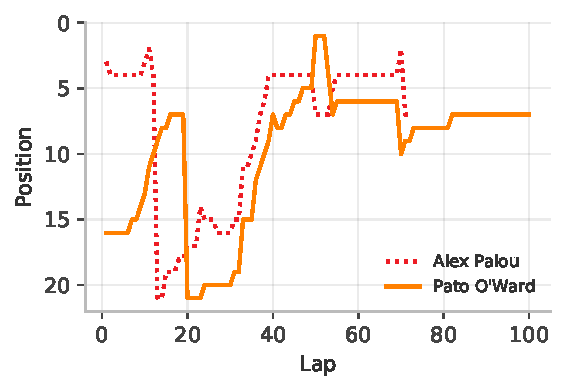
\includegraphics[keepaspectratio]{index_files/figure-pdf/cell-6-output-1.pdf}}
\end{center}

\textsubscript{Source:
\href{https://ArchithSharma.github.io/raceindycar_manuscript/index.qmd.html}{Article
Notebook}}

For example, \texttt{plot\_qualifying\_vs\_finish} is shown here. In
this case, Alex Palou crashed on lap 72, so he does not have a running
position afterwards.

Additionally, we can plot information for multiple races. For example,
\texttt{plot\_qualifying\_vs\_finish} is shown below the code chunk.
Other functions such as \texttt{plot\_position\_gain} and
\texttt{plot\_metric\_vs\_qualifying} are not shown for brevity's sake.

\textsubscript{Source:
\href{https://ArchithSharma.github.io/raceindycar_manuscript/index.qmd.html}{Article
Notebook}}

\begin{Shaded}
\begin{Highlighting}[]
\ImportTok{import}\NormalTok{ pandas }\ImportTok{as}\NormalTok{ pd}

\NormalTok{det26\_race }\OperatorTok{=}\NormalTok{ raceindycar.get\_session(}\DecValTok{2026}\NormalTok{, }\StringTok{"Detroit Grand Prix"}\NormalTok{, session}\OperatorTok{=}\StringTok{"R"}\NormalTok{)}
\NormalTok{det26\_race.load(laps}\OperatorTok{=}\VariableTok{True}\NormalTok{)}

\NormalTok{combined\_results }\OperatorTok{=}\NormalTok{ pd.concat([}
\NormalTok{    det25\_race.results.assign(Year}\OperatorTok{=}\DecValTok{2025}\NormalTok{),}
\NormalTok{    det26\_race.results.assign(Year}\OperatorTok{=}\DecValTok{2026}\NormalTok{)}
\NormalTok{])}

\CommentTok{\# Scatter of starting position vs finishing position with trend line}
\NormalTok{fig, ax }\OperatorTok{=}\NormalTok{ plotting.plot\_qualifying\_vs\_finish(}
\NormalTok{    combined\_results}
\NormalTok{)}
\NormalTok{fig.set\_size\_inches(}\DecValTok{4}\NormalTok{, }\FloatTok{2.5}\NormalTok{)}

\NormalTok{plt.show()}
\end{Highlighting}
\end{Shaded}

\begin{center}
\pandocbounded{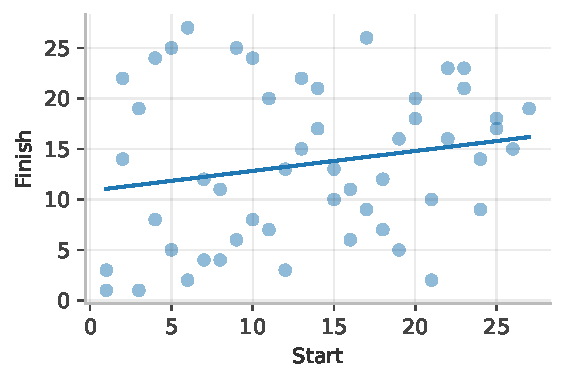
\includegraphics[keepaspectratio]{index_files/figure-pdf/cell-7-output-1.pdf}}
\end{center}

\textsubscript{Source:
\href{https://ArchithSharma.github.io/raceindycar_manuscript/index.qmd.html}{Article
Notebook}}

\subsection{Caching}\label{caching}

This library mirrors
\href{https://docs.fastf1.dev/api_reference/cache_and_rate_limits.html}{FastF1's
\texttt{Cache}} API, and there are two stages for caching.

The first stage uses an SQLite table to store HTTP requests and results
for \href{https://www.indycar.com/}{IndyCar}, which are rate-limited to
around one request per two seconds. The second stage stores Pickle/CSV
files that contain information from loading a race.

\textsubscript{Source:
\href{https://ArchithSharma.github.io/raceindycar_manuscript/index.qmd.html}{Article
Notebook}}

\begin{Shaded}
\begin{Highlighting}[]
\ImportTok{from}\NormalTok{ raceindycar.cache }\ImportTok{import}\NormalTok{ Cache}

\CommentTok{\# Enable Cache with specified directory using either pickle or csv format}
\NormalTok{raceindycar.enable\_cache(cache\_dir}\OperatorTok{=}\StringTok{".cache/raceindycar"}\NormalTok{, cache\_format}\OperatorTok{=}\StringTok{"pickle"}\NormalTok{)}

\CommentTok{\# Wipe Stage 2 (parsed/pickle) data, keeping the HTTP cache.}
\CommentTok{\# Optionally, wipe all Stage 1 HTTP requests with deep=True.}
\NormalTok{Cache.clear\_cache(deep}\OperatorTok{=}\VariableTok{False}\NormalTok{)}

\CommentTok{\# Never hit the network and only use cached data,}
\CommentTok{\# raising an error if the data is not found locally.}
\NormalTok{Cache.offline\_mode(}\VariableTok{True}\NormalTok{)}
\end{Highlighting}
\end{Shaded}

\textsubscript{Source:
\href{https://ArchithSharma.github.io/raceindycar_manuscript/index.qmd.html}{Article
Notebook}}

\subsection{Summary and Application}\label{summary-and-application}

Through utilizing official \href{https://www.indycar.com/}{IndyCar
data}, RaceIndyCar obtains session-level data, even down to individual
section times for every lap. We can store this information for reuse and
plot key metrics.

Applying this at a weekend level, we can see how qualifying lap times
associate with race lap times for individual drivers. On a multi-race
level, we can start to identify patterns and trends to create actionable
results, such as identifying optimal practice time, resource allocation
to adjusting the car from qualifying to race day, and more.

\section{Quantifying the Importance of Qualifying Across Race
Series}\label{quantifying-the-importance-of-qualifying-across-race-series}

Let \(Q_{ir}\), \(F_{ir}\) denote qualifying and finishing position for
driver \(i\) in race \(r\), and \(L_{ir\ell}\) the lap time on lap
\(\ell\).

\subsection{Pace Normalization}\label{pace-normalization}

Raw lap times are first converted to a race/lap-normalized pace score,

\begin{equation}\protect\phantomsection\label{eq-pace}{
z_{ir\ell} = \frac{L_{ir\ell} - \text{median}_j(L_{jr\ell})}{\text{sd}_j(L_{jr\ell})},
}\end{equation}

making pace comparable across tracks and eras.

\subsection{Driver and Team Quality}\label{driver-and-team-quality}

A race-level pace summary
\(\bar z_{ir} = \text{median}_\ell(z_{ir\ell})\) is then aggregated,
leave-one-race-out, into a driver quality score

\begin{equation}\protect\phantomsection\label{eq-driver-quality}{
\text{DQ}_{ir} = -\frac{1}{N_i-1}\sum_{r'\neq r}\bar z_{ir'},
}\end{equation}

sign-flipped so higher is better, with team quality \(\text{TQ}_{ir}\)
defined analogously. Excluding race \(r\) from its own quality estimate
is essential: including it would let a driver's result in \(r\) partly
explain itself, inflating quality's apparent explanatory power and
artificially shrinking qualifying's incremental contribution. Both
scores are then z-scored within series (\(\text{DQ}^z_{ir}\),
\(\text{TQ}^z_{ir}\), sample sd) so coefficients are comparable across
F1, IndyCar, and NASCAR despite each series having a different raw pace
scale.

\subsection{Regression Framework}\label{regression-framework}

The core analysis fits six nested OLS models per series, each with race
fixed effects \(\alpha_r\) to absorb track- and event-level
heterogeneity (weather, field size, caution frequency) so that
qualifying and quality are identified from within-race variation only:

\begin{equation}\protect\phantomsection\label{eq-models}{
\begin{aligned}
F_{ir} &= \alpha_r + \beta_1 Q_{ir} + \varepsilon_{ir} &&\text{(M1, qualifying only)}\\
F_{ir} &= \alpha_r + \gamma_1 \text{DQ}^z_{ir} + \varepsilon_{ir} &&\text{(M2, driver quality only)}\\
F_{ir} &= \alpha_r + \beta_2 Q_{ir} + \gamma_2 \text{DQ}^z_{ir} + \varepsilon_{ir} &&\text{(M3, both)}\\
F_{ir} &= \alpha_r + \delta_1 \text{TQ}^z_{ir} + \varepsilon_{ir} &&\text{(M4, team quality only)}\\
F_{ir} &= \alpha_r + \beta_3 Q_{ir} + \delta_2 \text{TQ}^z_{ir} + \varepsilon_{ir} &&\text{(M5, both)}\\
F_{ir} &= \alpha_r + \beta_4 Q_{ir} + \gamma_3 \text{DQ}^z_{ir} + \delta_3 \text{TQ}^z_{ir} + \varepsilon_{ir} &&\text{(M6, full)}
\end{aligned}
}\end{equation}

Reduced/full pairs (e.g., M2 vs.~M3) are always fit on an identical
common sample, so any R² difference reflects the added variable alone
rather than sample drift.

\subsection{Partial R²}\label{partial-ruxb2}

We report both the raw increment and the partial R²,

\begin{equation}\protect\phantomsection\label{eq-partial-r2}{
\Delta R^2 = R^2_F - R^2_R, \qquad
R^2_{\text{partial}} = \frac{R^2_F - R^2_R}{1-R^2_R},
}\end{equation}

with partial R² as the headline statistic because raw increments aren't
comparable across series with different baseline \(R^2_R\) --- a series
where quality already explains most of the variance has structurally
less room left for qualifying to add to, and the partial-R²
normalization removes that ceiling effect.

\subsection{Race-Level Analysis}\label{race-level-analysis}

To check the pooled estimate isn't driven by a handful of races, each
race is also fit independently,

\begin{equation}\protect\phantomsection\label{eq-race-level}{
F_{ir} = \alpha_r^{(0)} + \beta_r Q_{ir} + \varepsilon_{ir},
}\end{equation}

yielding a \emph{distribution} of race-level \(R^2_r\) rather than one
pooled number, alongside per-race and pooled Spearman's \(\rho\) as a
distribution-free complement to the linear \(\beta_r\). Linear OLS is
preferred over rank-based or ordinal alternatives throughout because it
yields additive, directly interpretable R² decompositions --- the
mechanism the incremental/partial-R² comparisons depend on --- while
Spearman correlation serves only as a robustness check on the same
relationship, not a replacement for it.

\section{Results}\label{sec-results}

Through our method, we find that position is a meaningful but partial
predictor of race outcome, and its importance varies sharply by series.
After conditioning on race fixed effects and each driver's underlying
pace, qualifying position still adds real explanatory power in all three
series, while the size of that effect differs by roughly a factor of two
to three between F1 and NASCAR.

\subsection{Qualifying and Finishing
Position}\label{qualifying-and-finishing-position}

First, we examine how qualifying position relates to finishing position
across the three series. We also look at the amount of position changes
that occur from qualifying to finish, which is a proxy for how much
variance there is in the race itself.

Figure~\ref{fig-quali-eda} shows that, in F1, high starting positions
have a higher average finish position than in the other two series.
However, this advantage compared to IndyCar ends at around position 7.
NASCAR's curve is flatter compared to the other two series, indicating
that average finish positions for many starting positions are similar.

\begin{figure}[H]

\begin{minipage}[t]{0.50\linewidth}

\centering{

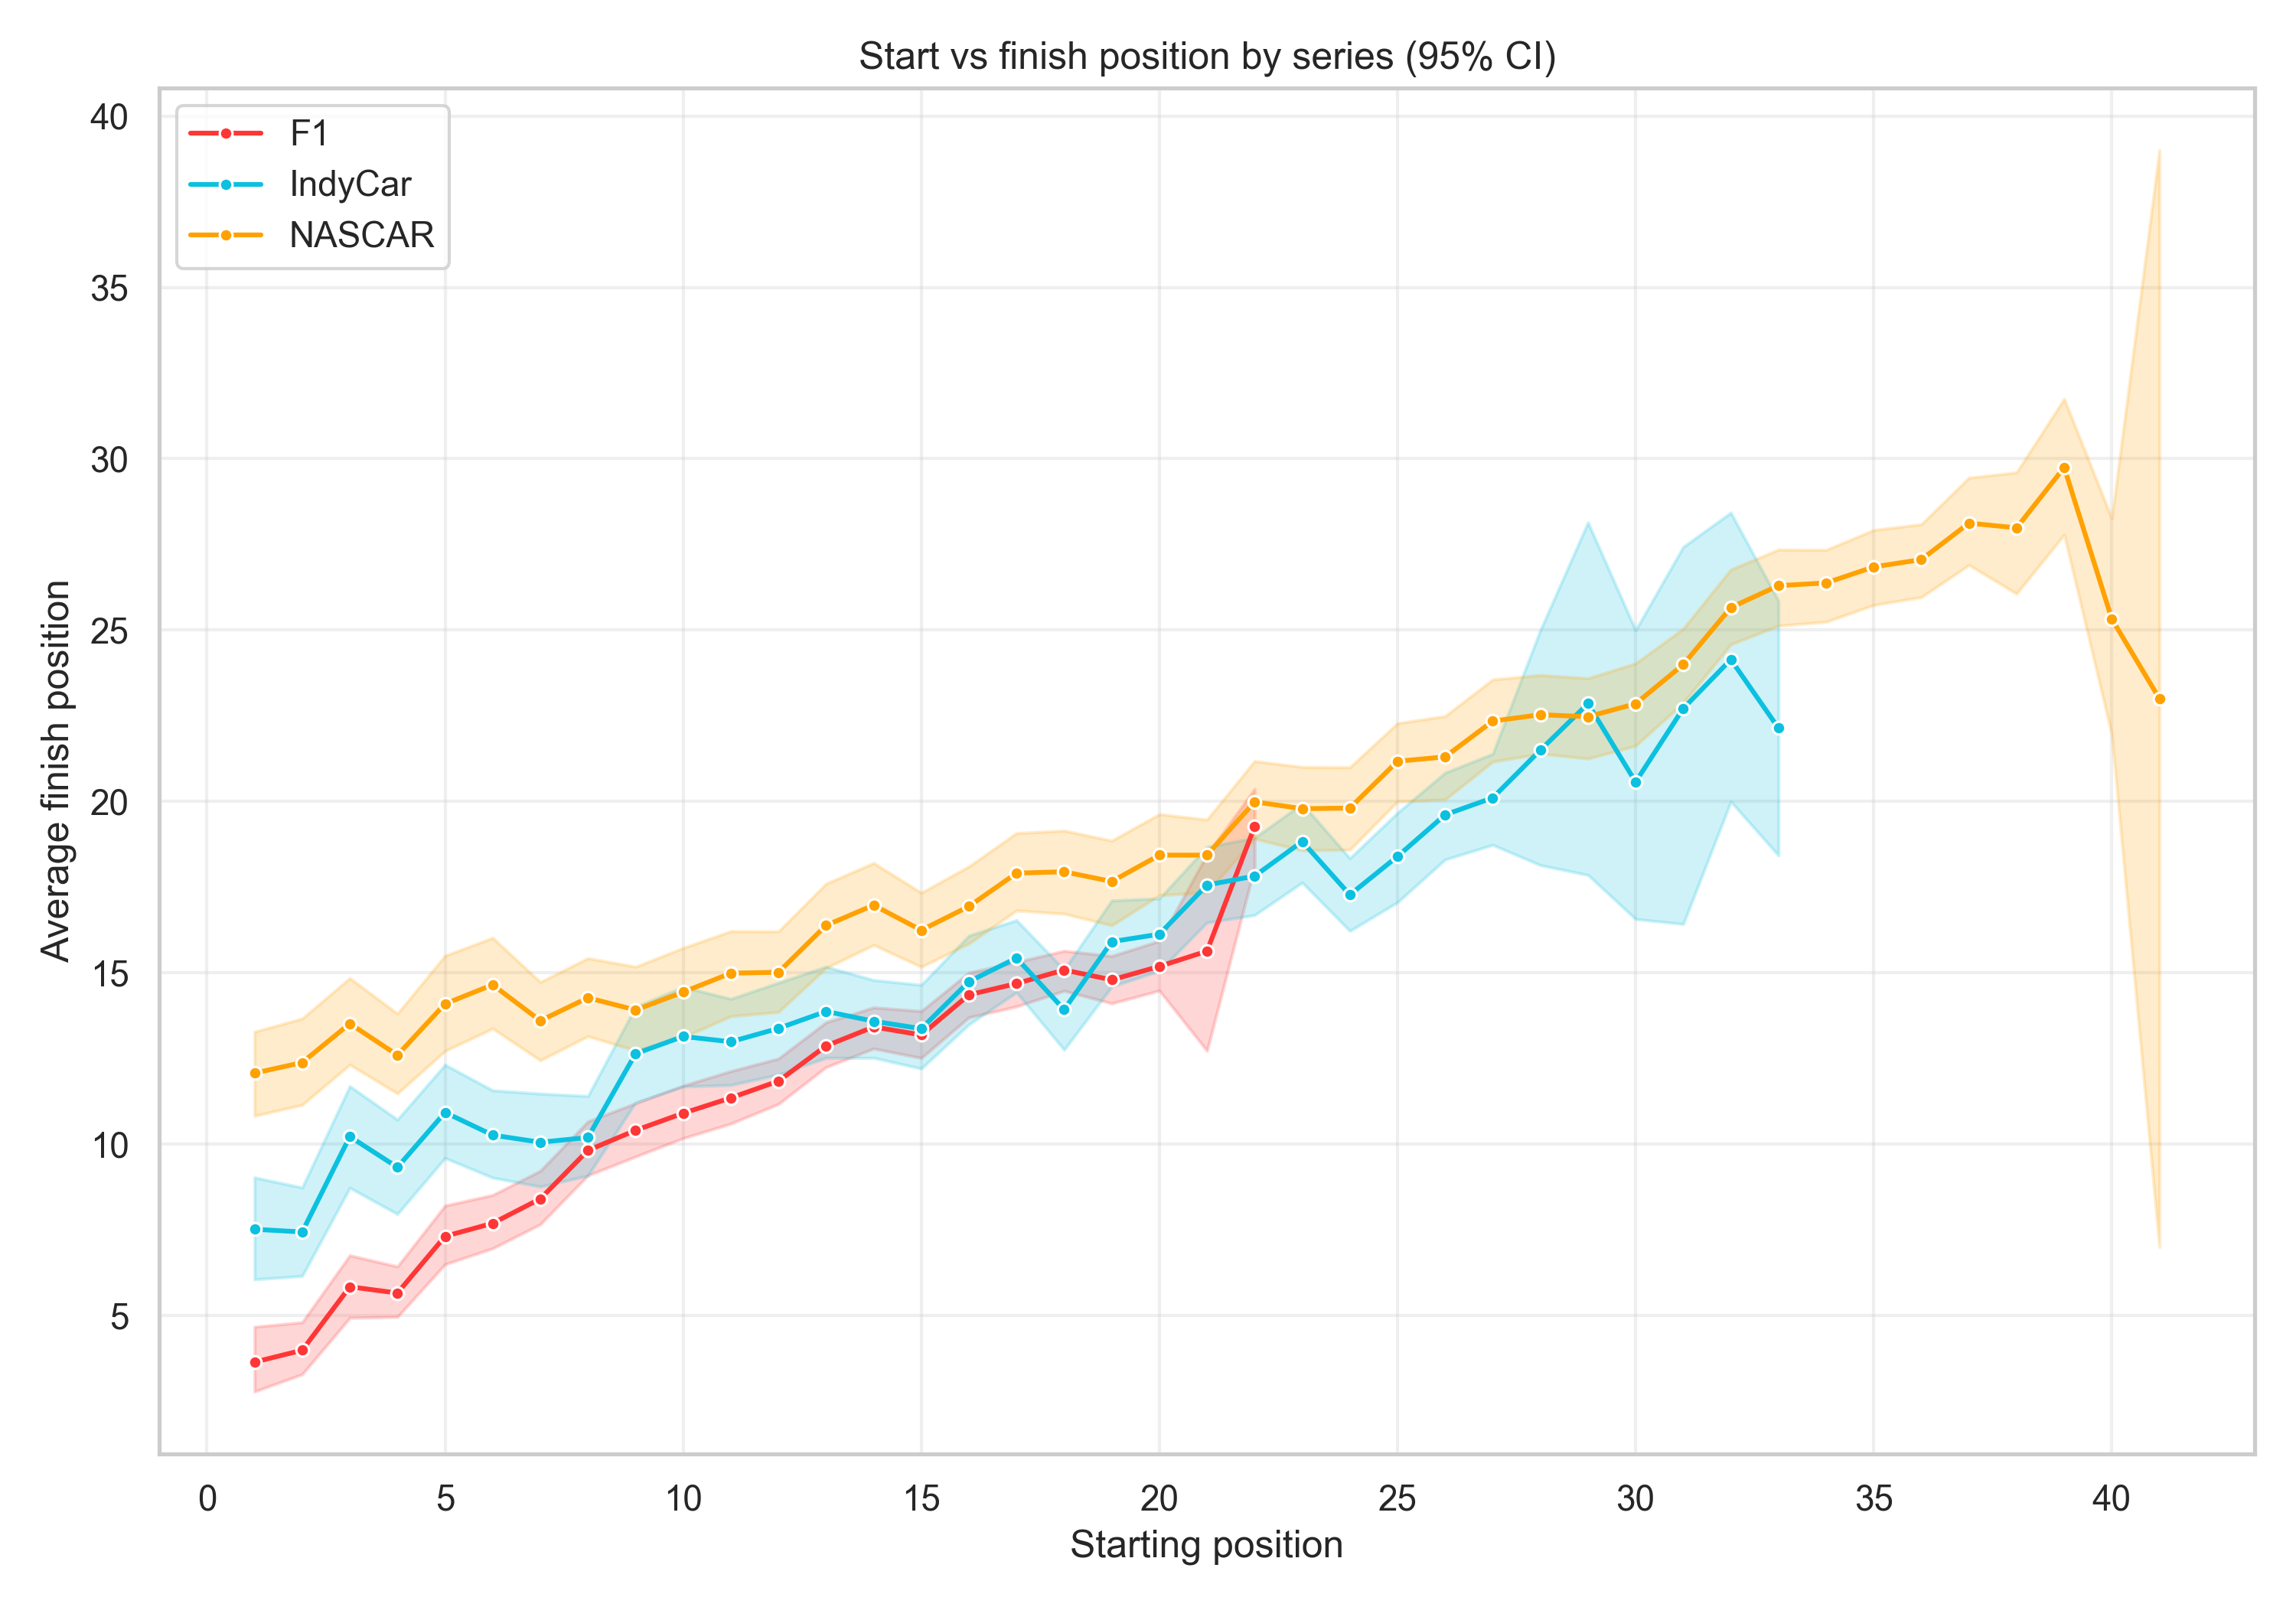
\includegraphics[width=0.6\linewidth,height=\textheight,keepaspectratio]{qualifying_importance_analysis/start_finish_by_series.png}

}

\subcaption{\label{fig-quali-eda}Qualifying position vs.~finishing
position, by series.}

\end{minipage}%
%
\begin{minipage}[t]{0.50\linewidth}

\centering{

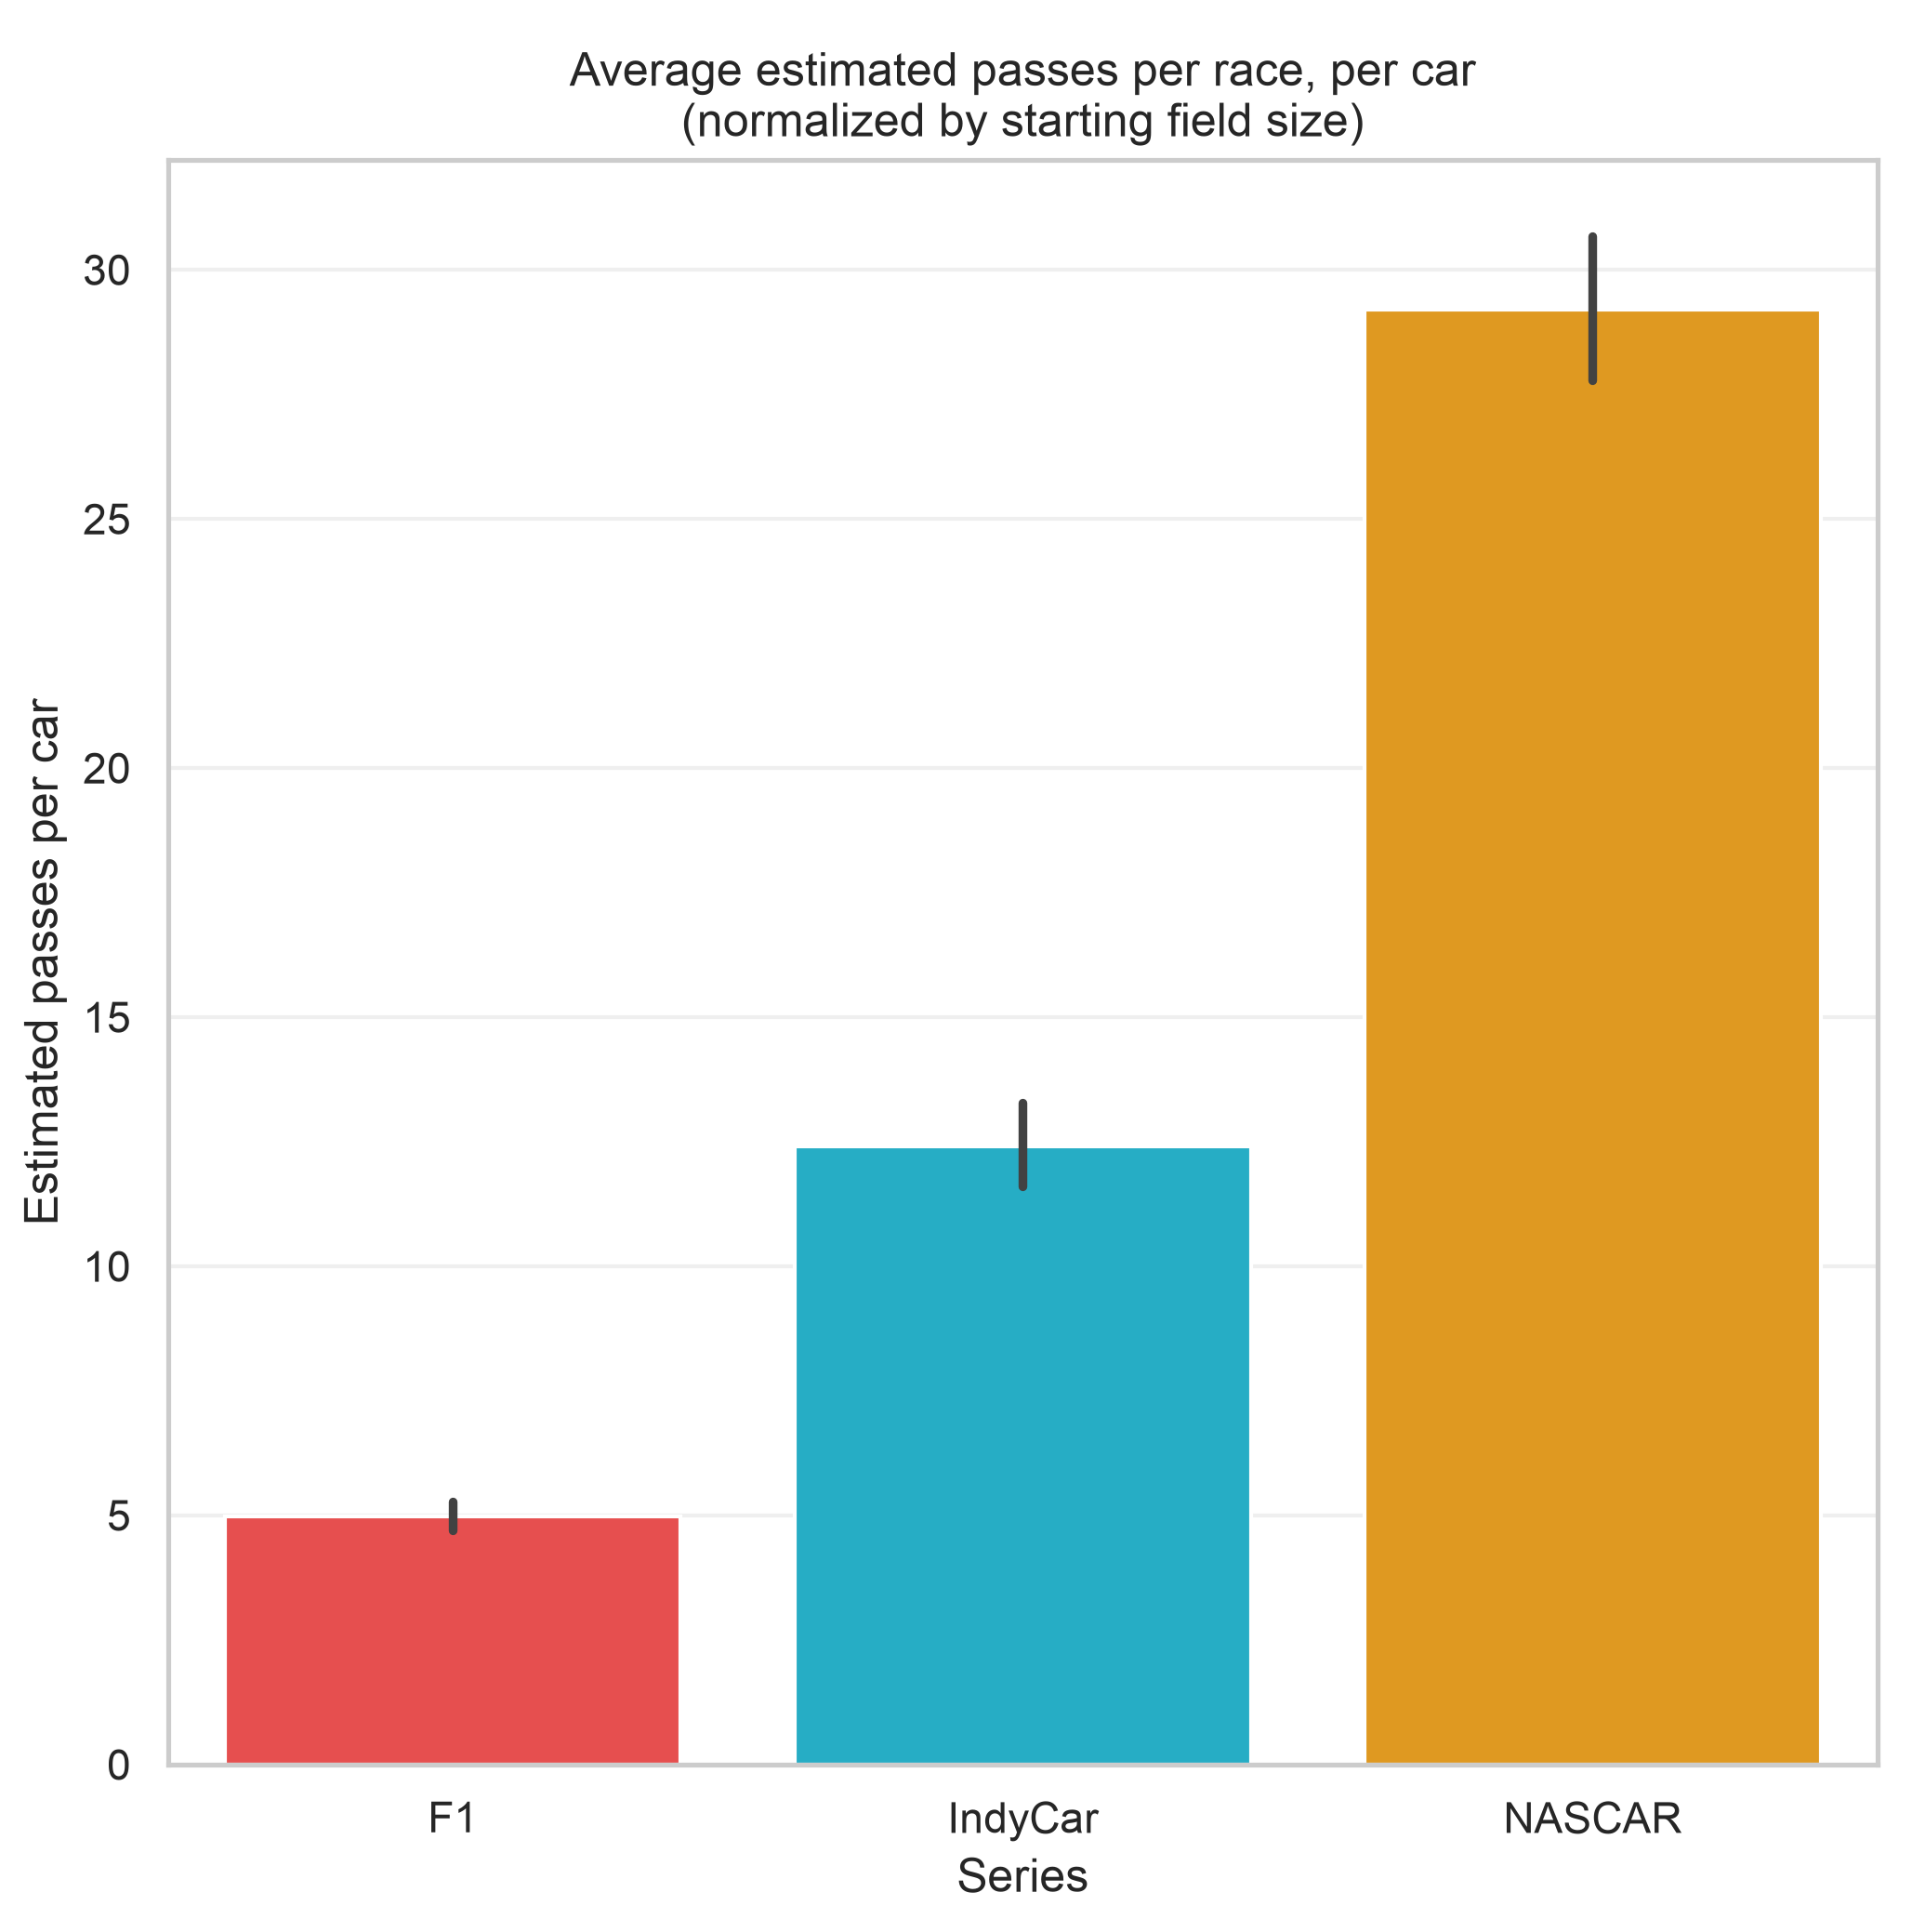
\includegraphics[width=0.6\linewidth,height=\textheight,keepaspectratio]{qualifying_importance_analysis/passes_per_race.png}

}

\subcaption{\label{fig-passes-eda}Normalized passes per race.}

\end{minipage}%

\caption{\label{fig-eda-raw}EDA of qualifying position vs.~finishing
position and passes per race}

\end{figure}%

In addition, each NASCAR driver performs approximately 6 times as many
passes as an F1 driver and over double the number for IndyCar drivers.

The scatter of qualifying position against finishing position
(Figure~\ref{fig-quali-finish}) shows a clear positive slope in all
three series, but with very different amounts of scatter around it. F1's
cloud is tightest and most linear; IndyCar and NASCAR show substantially
more vertical spread at every starting position, consistent with more
frequent late-race reshuffling (strategy, cautions, pit-stop variance)
loosening the grid-to-finish relationship. This is echoed in the
position-gain histograms (Figure~\ref{fig-position-gain}): F1 drivers
cluster tightly around ``no change'' from qualifying to finish, while
IndyCar and especially NASCAR show wide, roughly symmetric distributions
of gains and losses spanning ±20 to ±40 positions --- a signature of
much higher in-race variance.

\begin{figure}[H]

\begin{minipage}[t]{0.50\linewidth}

\centering{

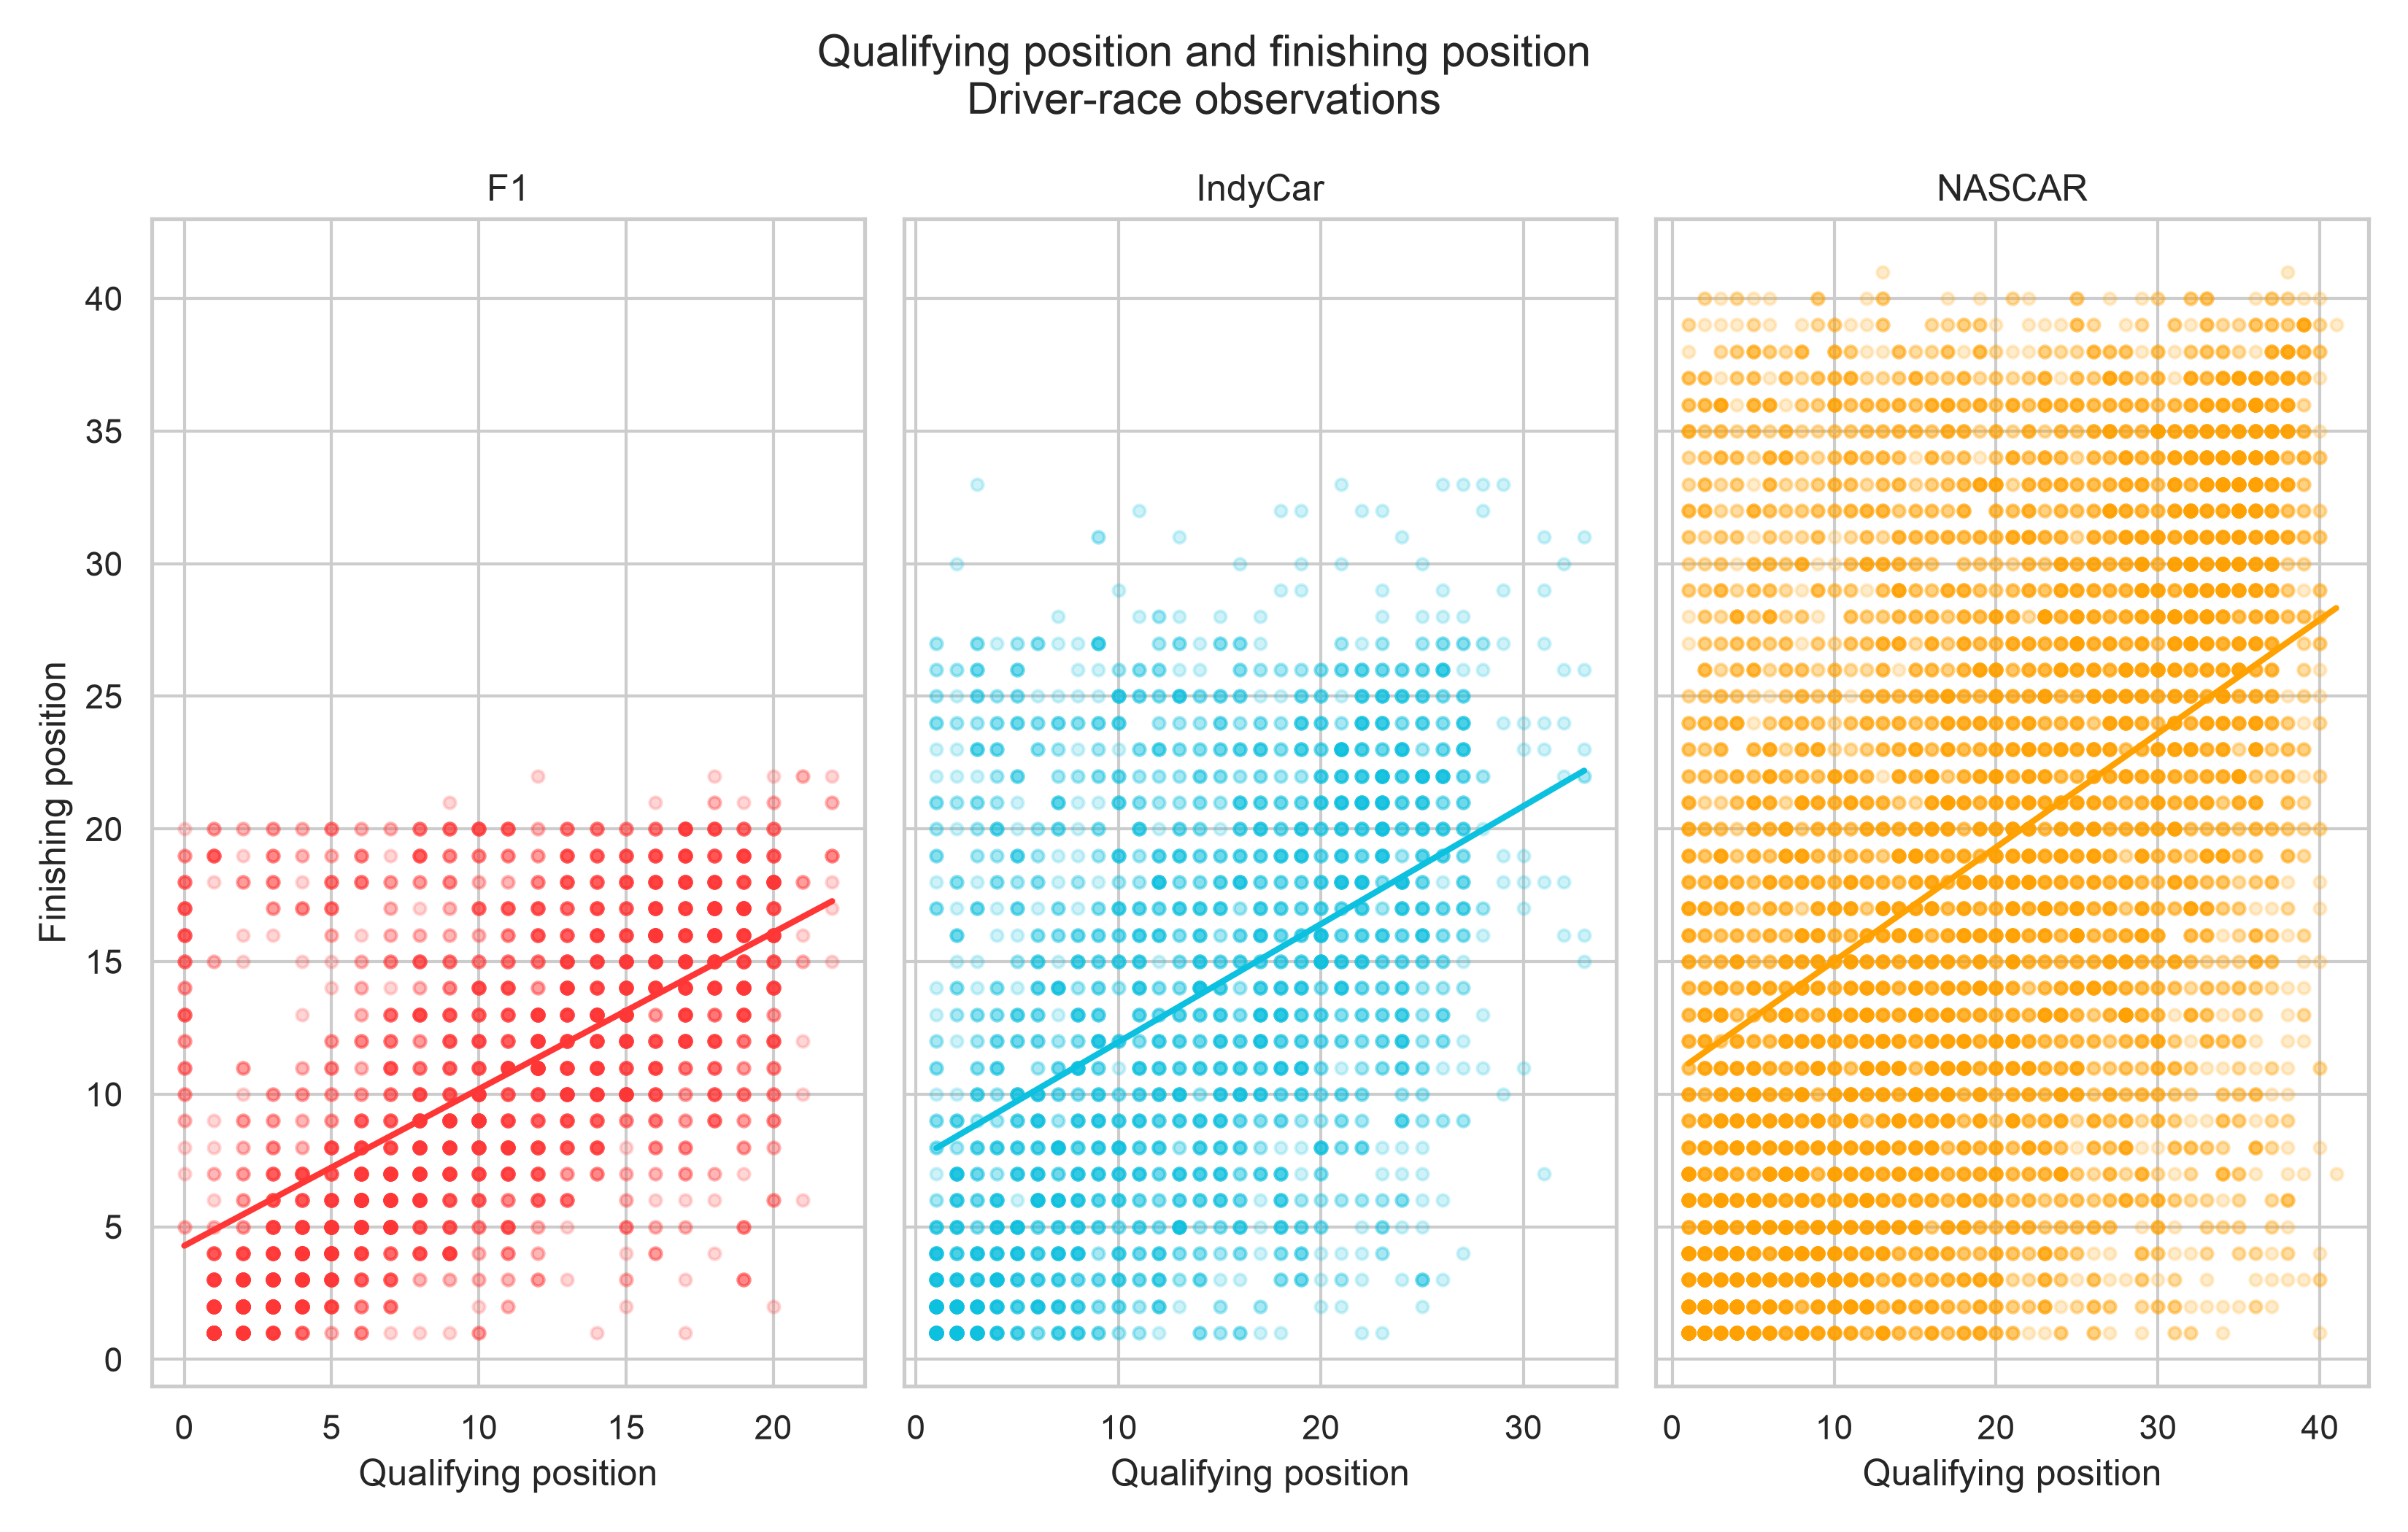
\includegraphics[width=0.6\linewidth,height=\textheight,keepaspectratio]{qualifying_importance_analysis/01_qualifying_vs_finish.png}

}

\subcaption{\label{fig-quali-finish}Qualifying position vs.~finishing
position, by series.}

\end{minipage}%
%
\begin{minipage}[t]{0.50\linewidth}

\centering{

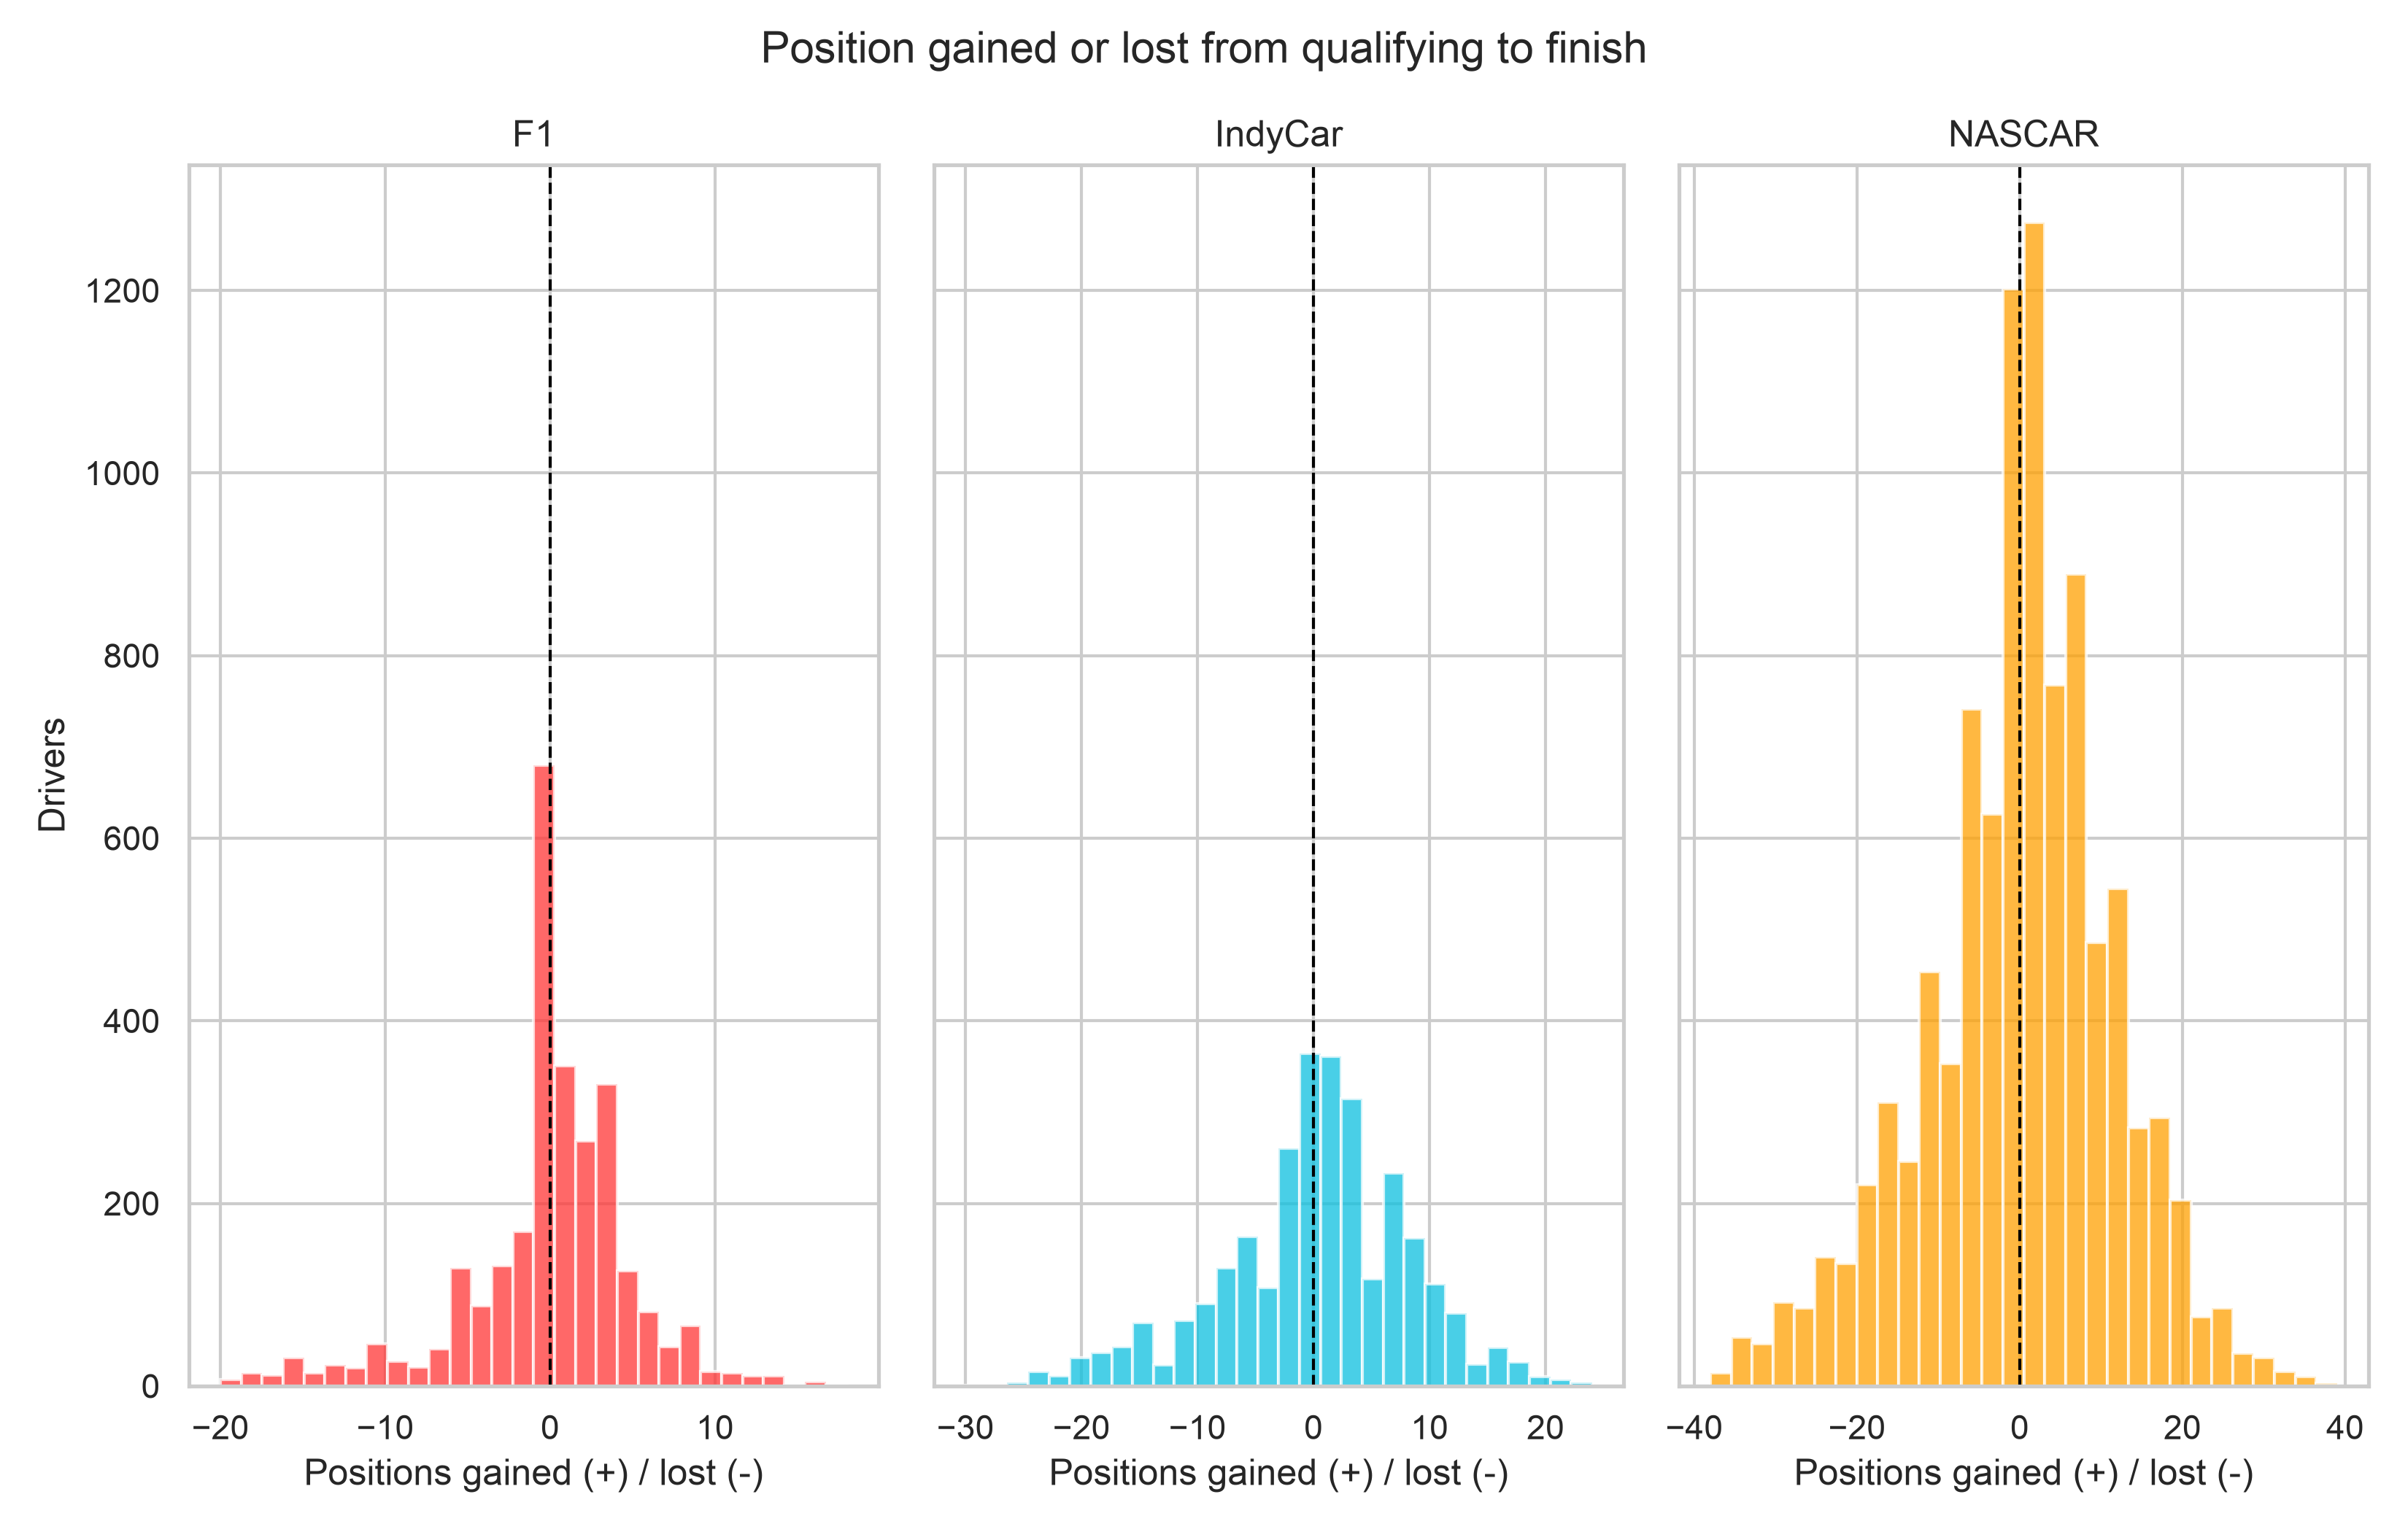
\includegraphics[width=0.6\linewidth,height=\textheight,keepaspectratio]{qualifying_importance_analysis/02_position_gain.png}

}

\subcaption{\label{fig-position-gain}Distribution of positions gained or
lost from qualifying to finish.}

\end{minipage}%

\caption{\label{fig-raw}Raw relationship between starting and finishing
position across series.}

\end{figure}%

\subsection{Adjusted Qualifying
Importance}\label{adjusted-qualifying-importance}

Using the common-sample specification
(\texttt{finish\ \textasciitilde{}\ driver\_quality\_z\ +\ race\ FE}
vs.~\texttt{finish\ \textasciitilde{}\ qualifying\ +\ driver\_quality\_z\ +\ race\ FE},
identical observations in both models):

\begin{longtable}[]{@{}
  >{\raggedright\arraybackslash}p{(\linewidth - 12\tabcolsep) * \real{0.0886}}
  >{\raggedleft\arraybackslash}p{(\linewidth - 12\tabcolsep) * \real{0.0633}}
  >{\raggedleft\arraybackslash}p{(\linewidth - 12\tabcolsep) * \real{0.0633}}
  >{\raggedleft\arraybackslash}p{(\linewidth - 12\tabcolsep) * \real{0.2278}}
  >{\raggedleft\arraybackslash}p{(\linewidth - 12\tabcolsep) * \real{0.2405}}
  >{\raggedleft\arraybackslash}p{(\linewidth - 12\tabcolsep) * \real{0.1899}}
  >{\raggedleft\arraybackslash}p{(\linewidth - 12\tabcolsep) * \real{0.1266}}@{}}
\caption{Common-sample qualifying incremental/partial R², controlling
for driver quality and race fixed
effects.}\label{tbl-common-sample}\tabularnewline
\toprule\noalign{}
\begin{minipage}[b]{\linewidth}\raggedright
Series
\end{minipage} & \begin{minipage}[b]{\linewidth}\raggedleft
n
\end{minipage} & \begin{minipage}[b]{\linewidth}\raggedleft
Races
\end{minipage} & \begin{minipage}[b]{\linewidth}\raggedleft
R² (quality only)
\end{minipage} & \begin{minipage}[b]{\linewidth}\raggedleft
R² (+ qualifying)
\end{minipage} & \begin{minipage}[b]{\linewidth}\raggedleft
Incremental R²
\end{minipage} & \begin{minipage}[b]{\linewidth}\raggedleft
Partial R²
\end{minipage} \\
\midrule\noalign{}
\endfirsthead
\toprule\noalign{}
\begin{minipage}[b]{\linewidth}\raggedright
Series
\end{minipage} & \begin{minipage}[b]{\linewidth}\raggedleft
n
\end{minipage} & \begin{minipage}[b]{\linewidth}\raggedleft
Races
\end{minipage} & \begin{minipage}[b]{\linewidth}\raggedleft
R² (quality only)
\end{minipage} & \begin{minipage}[b]{\linewidth}\raggedleft
R² (+ qualifying)
\end{minipage} & \begin{minipage}[b]{\linewidth}\raggedleft
Incremental R²
\end{minipage} & \begin{minipage}[b]{\linewidth}\raggedleft
Partial R²
\end{minipage} \\
\midrule\noalign{}
\endhead
\bottomrule\noalign{}
\endlastfoot
F1 & 2,778 & 142 & 0.339 & 0.451 & 0.113 & \textbf{0.170} \\
IndyCar & 2,908 & 113 & 0.218 & 0.272 & 0.054 & \textbf{0.069} \\
NASCAR & 9,695 & 272 & 0.226 & 0.258 & 0.032 & \textbf{0.042} \\
\end{longtable}

Qualifying explains roughly \textbf{17\% of the finishing-position
variance left unexplained by driver quality in F1}, versus about
\textbf{7\% in IndyCar} and \textbf{4\% in NASCAR}. The same ordering
holds under the team-quality specification
(Figure~\ref{fig-partial-r2}): partial R² for qualifying is 0.154 (F1),
0.110 (IndyCar), and 0.050 (NASCAR). Figure~\ref{fig-quali-vs-quality}
makes the driver-quality-vs-qualifying comparison directly: in F1,
qualifying alone carries roughly as much unadjusted explanatory weight
as driver quality; in IndyCar and NASCAR, driver quality's incremental
contribution meets or exceeds qualifying's.

\begin{figure}[H]

\begin{minipage}[t]{0.50\linewidth}

\centering{

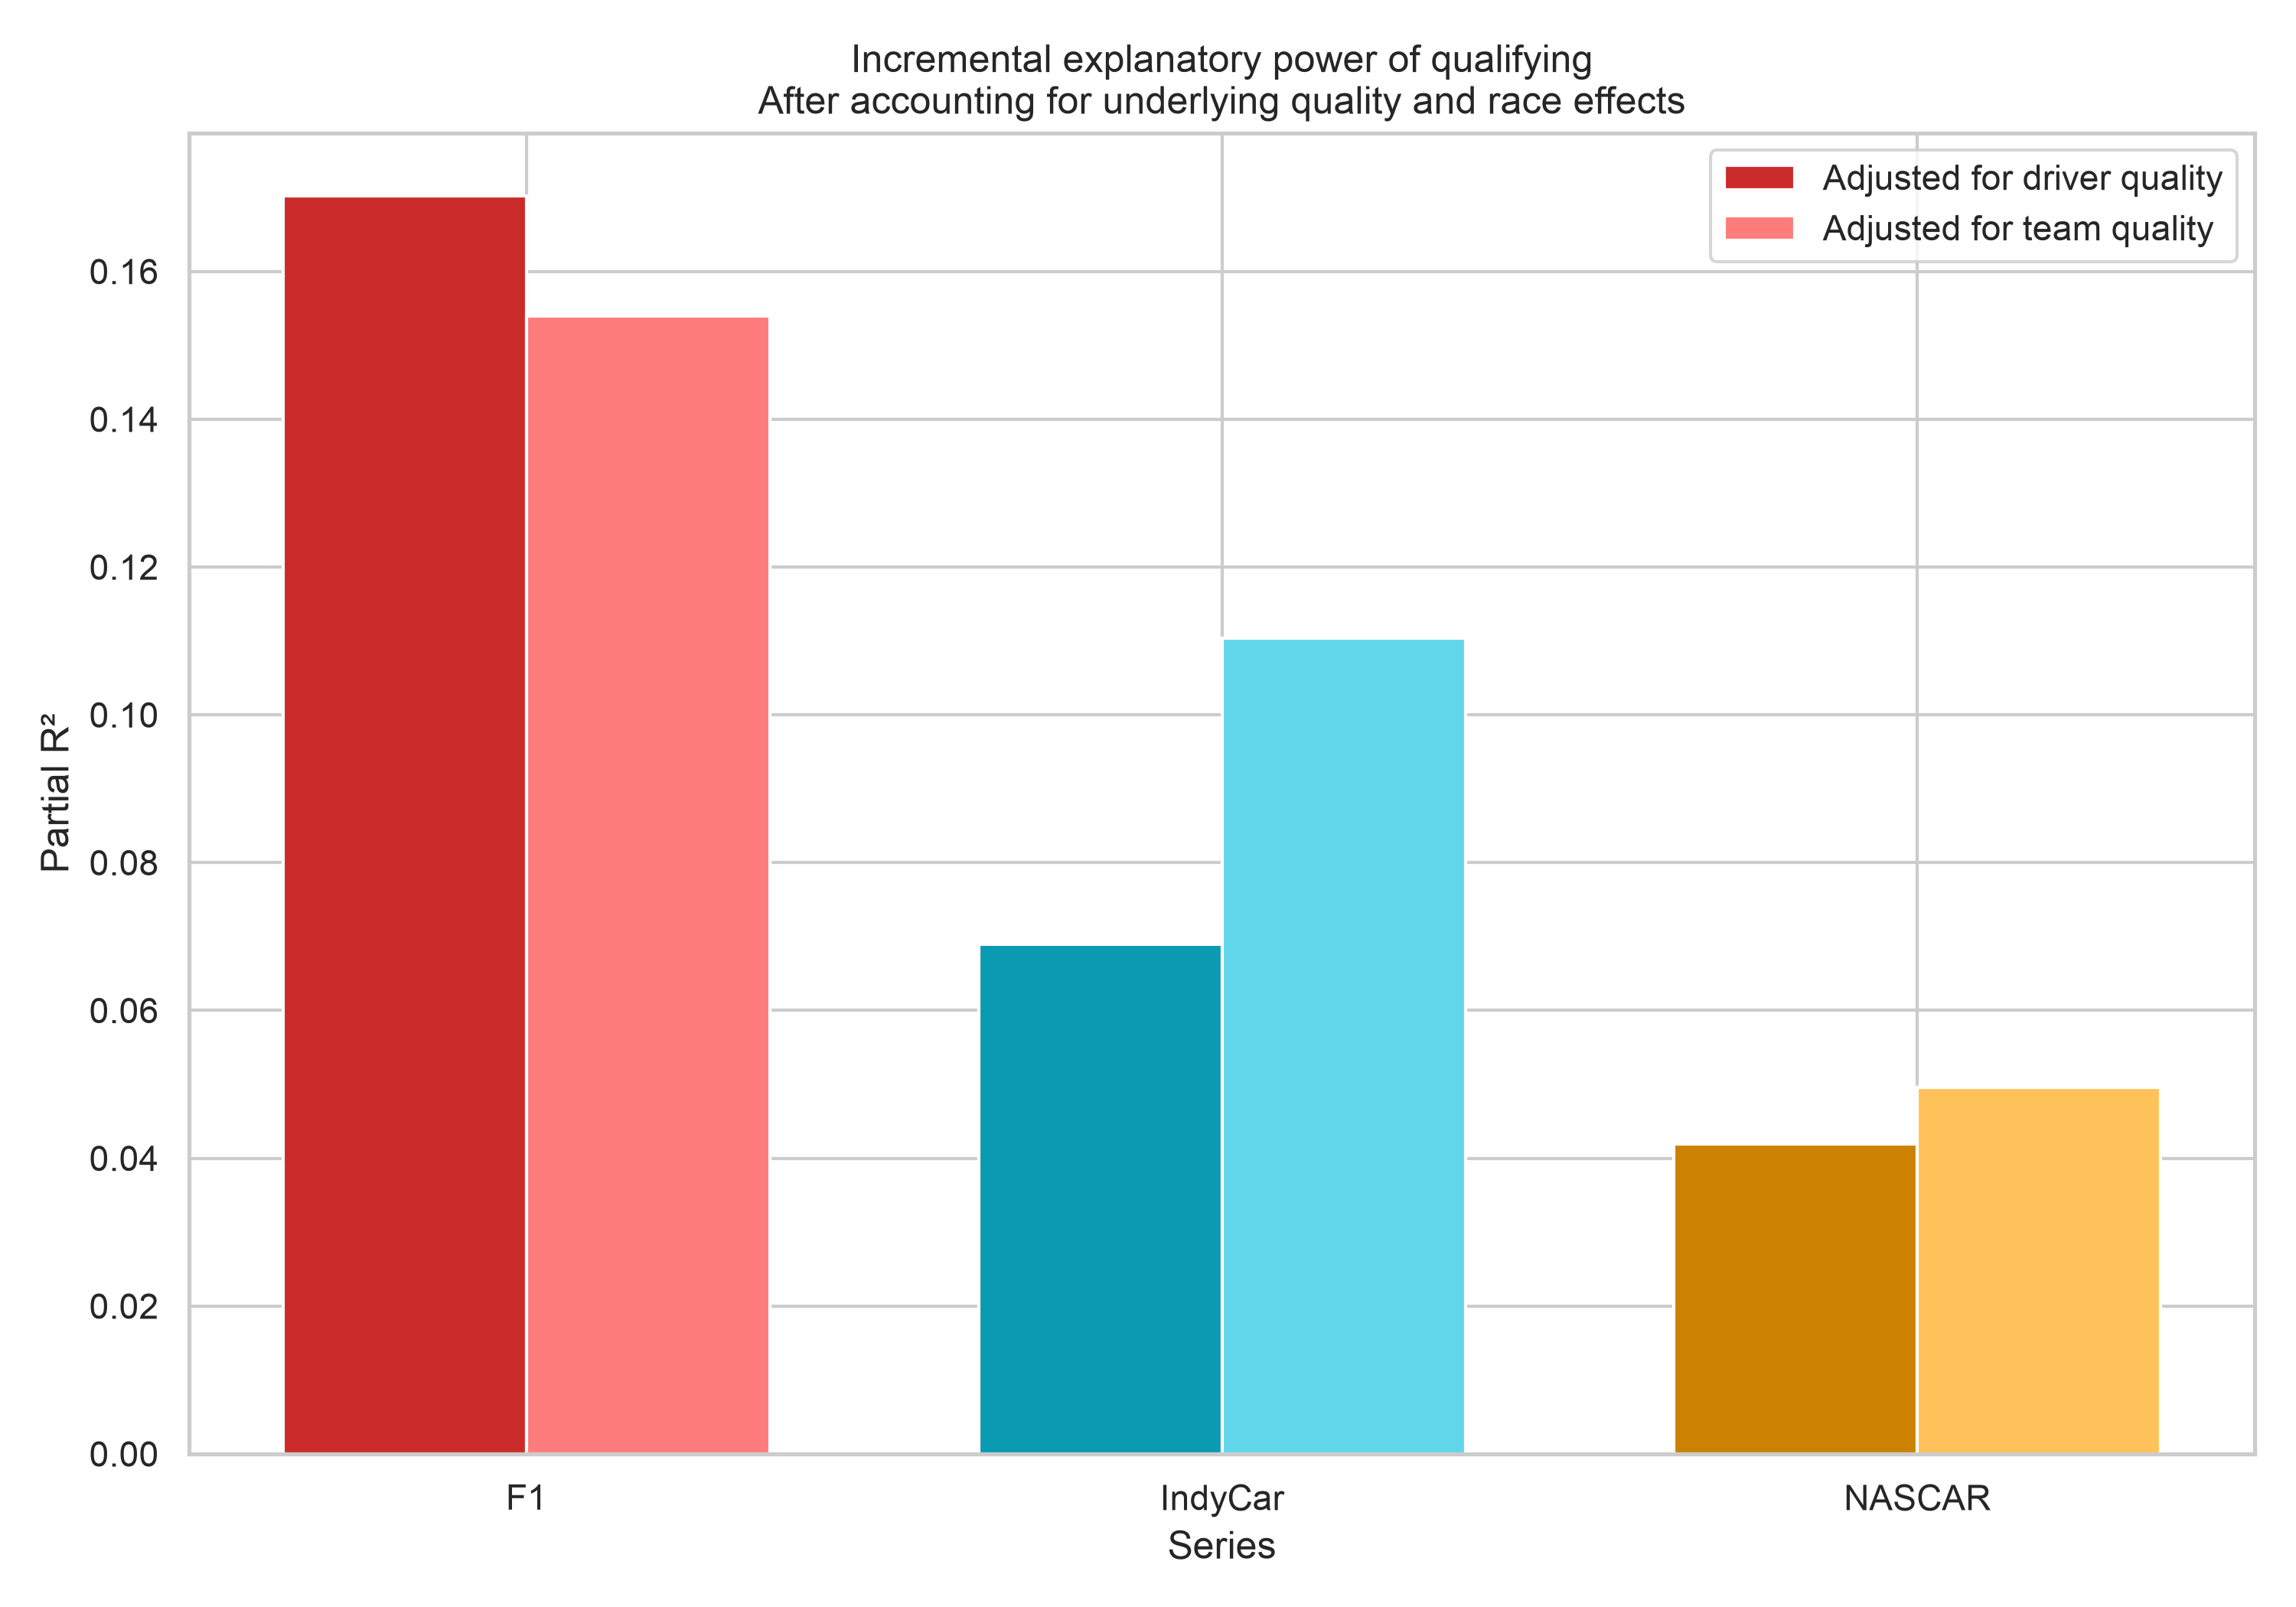
\includegraphics[width=0.6\linewidth,height=\textheight,keepaspectratio]{qualifying_importance_analysis/03_qualifying_partial_r2.png}

}

\subcaption{\label{fig-partial-r2}Incremental explanatory power of
qualifying, adjusted for driver and team quality.}

\end{minipage}%
%
\begin{minipage}[t]{0.50\linewidth}

\centering{

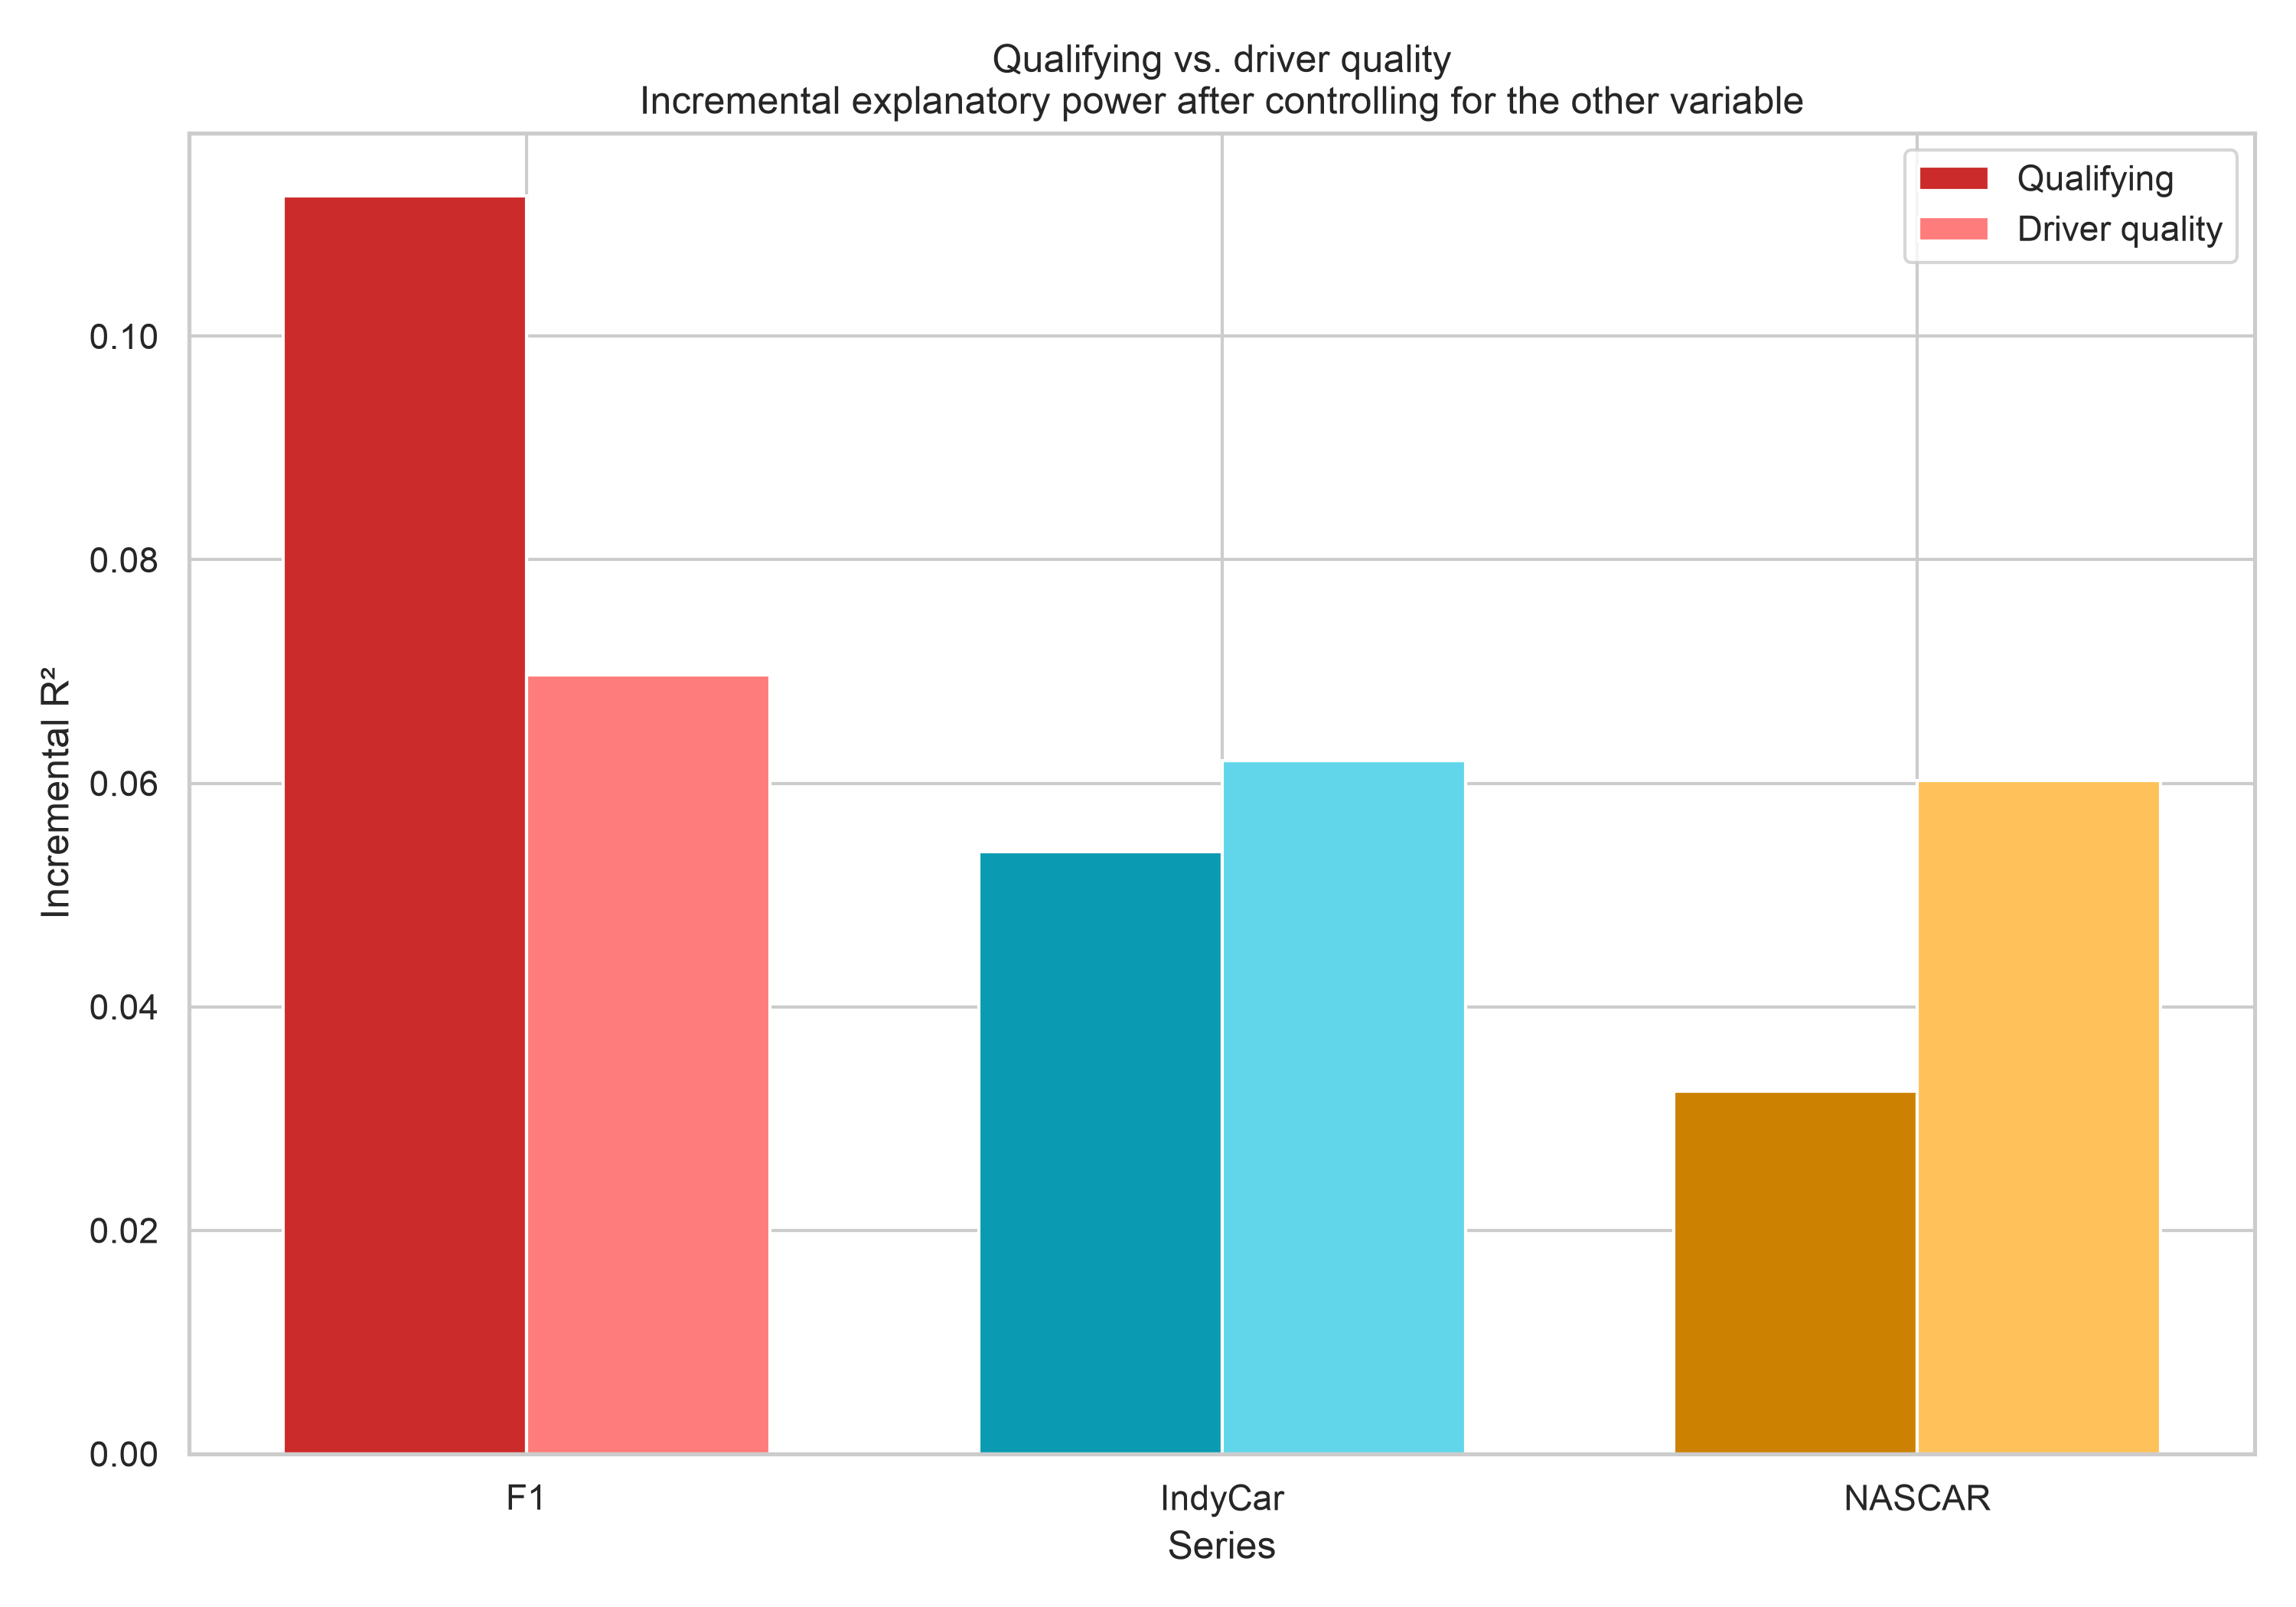
\includegraphics[width=0.6\linewidth,height=\textheight,keepaspectratio]{qualifying_importance_analysis/04_qualifying_vs_quality.png}

}

\subcaption{\label{fig-quali-vs-quality}Qualifying vs.~driver quality:
incremental R² controlling for the other variable.}

\end{minipage}%

\caption{\label{fig-r2-comparisons}Qualifying's incremental explanatory
power compared against underlying driver and team quality.}

\end{figure}%

Figure~\ref{fig-quality-vs-quali} confirms why quality and qualifying
are related but not redundant: driver quality (leave-one-race-out
relative pace) correlates negatively with qualifying position in all
three series (higher quality → better/lower grid slot), most steeply in
NASCAR and IndyCar and more moderately in F1. Because faster drivers
tend to qualify better, some of qualifying's predictive power is really
quality, which is exactly what the driver-quality control is designed to
strip out. That qualifying still retains independent explanatory power
after this adjustment (particularly in F1) indicates that grid position
carries information beyond who's fastest on a given weekend --- most
plausibly \emph{track-position value}: the tactical advantage of racing
near the front (clean air, fewer overtakes required, less exposure to
pack incidents), which matters more where passing is harder (F1) and
less where it's easier or where race-day variance dominates (NASCAR, and
to a lesser extent IndyCar).

\begin{figure}[H]

\centering{

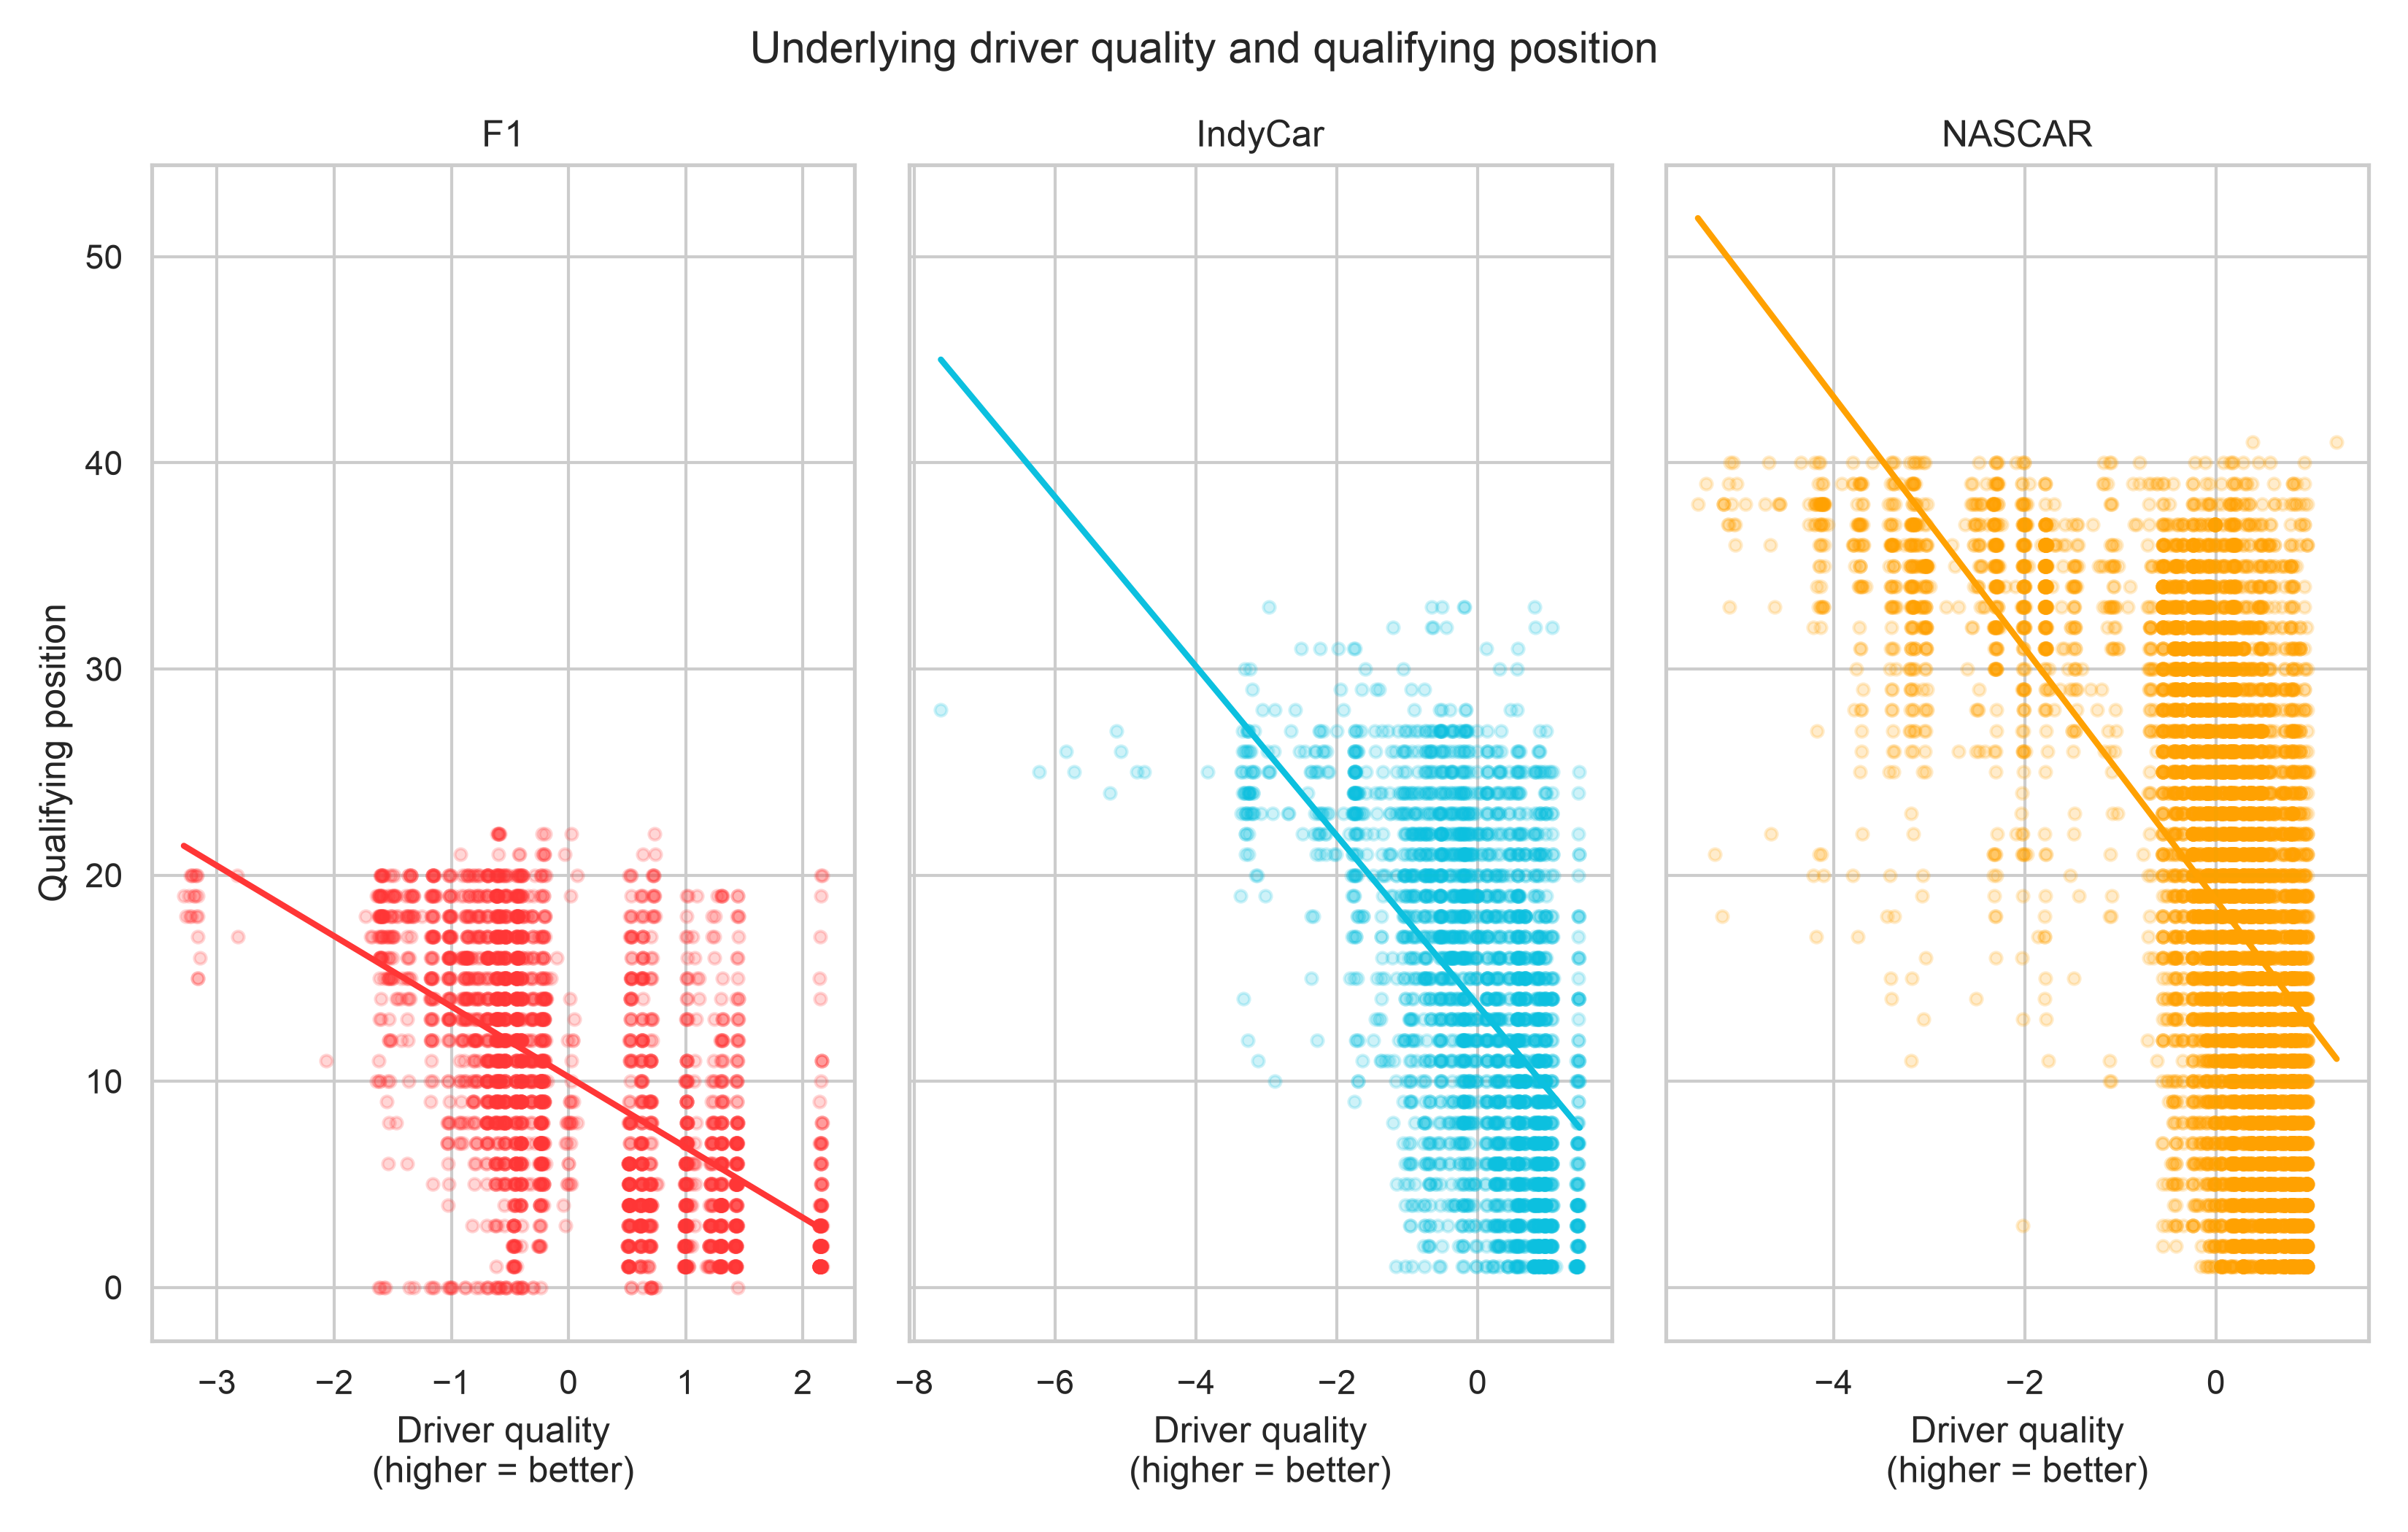
\includegraphics[width=0.6\linewidth,height=\textheight,keepaspectratio]{qualifying_importance_analysis/06_quality_vs_qualifying.png}

}

\caption{\label{fig-quality-vs-quali}Underlying driver quality
vs.~qualifying position, by series.}

\end{figure}%

\subsection{Race-Level Variation}\label{race-level-variation}

Figure~\ref{fig-race-level} shows the distribution of race-level R² (a
separate qualifying → finish regression fit within each individual race,
no pooling). F1's median race-level R² (\textasciitilde0.41) is roughly
double IndyCar's (\textasciitilde0.21) and more than double NASCAR's
(\textasciitilde0.18), and F1's IQR sits noticeably higher on the axis.
NASCAR shows the widest and most left-skewed spread, with many
individual races near R² ≈ 0, which is consistent with our EDA findings
of frequent reshuffling and high in-race variance.

\begin{figure}[H]

\centering{

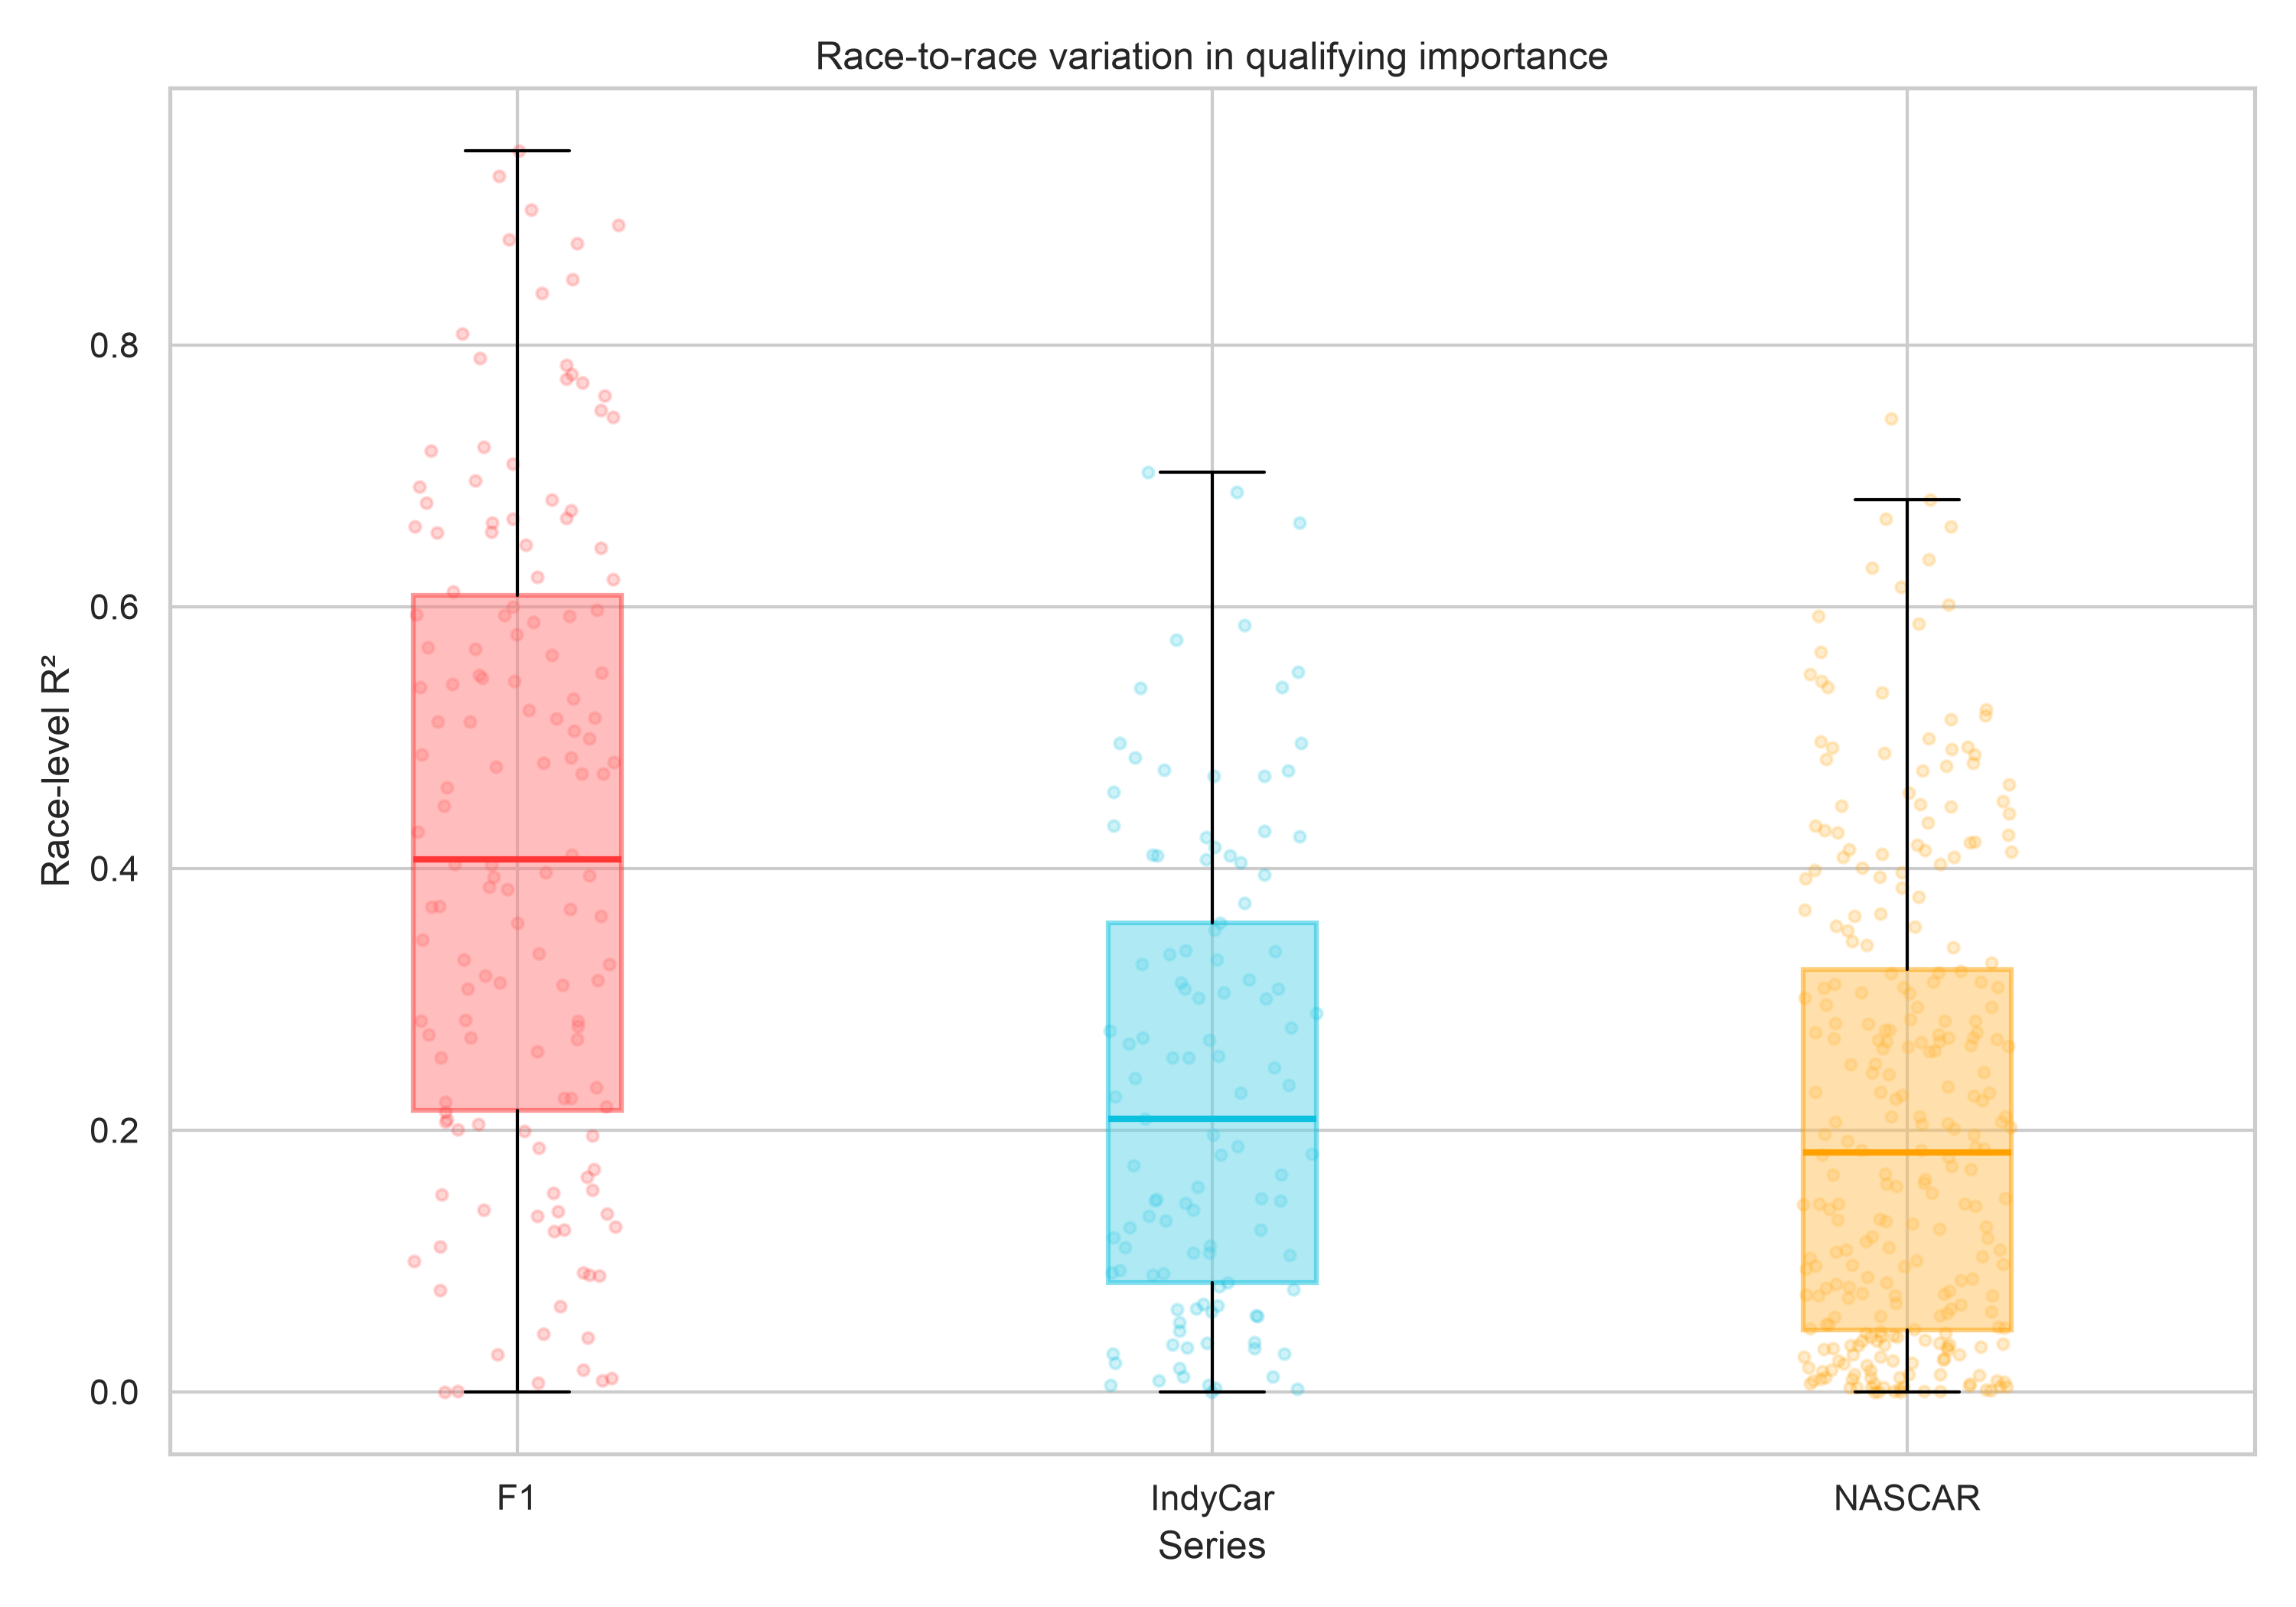
\includegraphics[width=0.7\linewidth,height=\textheight,keepaspectratio]{qualifying_importance_analysis/05_race_level_qualifying_r2.png}

}

\caption{\label{fig-race-level}Race-to-race variation in qualifying
importance (race-level R², no pooling).}

\end{figure}%

\subsection{Qualifying and Lap 1
Position}\label{qualifying-and-lap-1-position}

As a secondary check, qualifying position correlates very strongly with
observed Lap 1 running position (Pearson r = 0.81 F1, 0.92 IndyCar, 0.92
NASCAR). However, using Lap 1 position instead of qualifying position as
the predictor yields even larger partial R² values --- 0.257 (F1), 0.087
(IndyCar), 0.048 (NASCAR) --- suggesting that whilst qualifying is
important, there is a lot of information that is uncovered from Lap 1
variance.

\section{Discussion}\label{discussion}

Qualifying proves to have a statistically significant predictor of
finish position, adjusting for race performance. However, this effect
decreases in magnitude from F1 to IndyCar to NASCAR.

Motorsport viewers can take this information to inform decisions about
what to watch on a race weekend. For F1 fans, compared to NASCAR or
IndyCar fans, because 17\% of the variability in finish position not
explained by driver skill can be explained by qualifying position, it is
more important to tune in to qualifying sessions because of its
importance to race day. It also gives NASCAR and IndyCar fans more hope
for their drivers who qualify poorly, as it only accounts for 4 and 6
percent of the aforementioned variability.

Additionally, these results can inform new viewers about their desired
series to watch, and for the series themselves, what events they can
market. If a viewer enjoys watching qualifying and having a large time
investment in watching a race series, then perhaps F1 is the series to
watch for them, as it has a larger effect on race day results than
IndyCar or NASCAR. On the other hand, if they only want to watch an
exciting race, then IndyCar and/or NASCAR is the way to go because there
is more variance in finish position from start position, meaning there
is more passing and more excitement for the viewer on a lap-by-lap
basis. This is supported by the average number of passes for F1,
IndyCar, and NASCAR races, which are 5, 12, and 29, respectively.

For the same reasons, F1 teams, relative to NASCAR and IndyCar teams,
should be putting more effort into creating a solid qualifying
performance because it appears to have a larger effect on race results.

As a corollary, while qualifying is important, lap one running position
is significantly more important for F1 drivers compared to IndyCar and
NASCAR, as the difference in the predictive value for qualifying
position and lap one position is 8.7\%, 1.8\%, and 0.6\%, respectively.
These drivers can take a more relaxed approach to the first lap, as it
is not devastating to informing race results.

\section{Limitations and Future Work}\label{limitations-and-future-work}

Differing weather conditions between qualifying and race day were not
accounted for in this analysis. For the future, incorporating weather
into the analysis can inform teams on how to adjust strategy based on
varying conditions. We also did not create a function for teams to
identify specifically the impact of adjustments for specific scenarios.
For example, it would be helpful for a team to know if an \(x\) increase
in race speed for a \(y\) position trade-off in qualifying will be worth
it because they will gain back those lost positions.

\section{Conclusion}\label{conclusion}

Overall, this project creates new opportunities for data analytics in
the IndyCar realm through the RaceIndyCar package and offers a novel
method of comparing races across series through our numerical analysis.

\textsubscript{Source:
\href{https://ArchithSharma.github.io/raceindycar_manuscript/index.qmd.html}{Article
Notebook}}


\bibliography{references.bib}



\end{document}
